\documentclass[11pt]{article}

    \usepackage[breakable]{tcolorbox}
    \usepackage{parskip} % Stop auto-indenting (to mimic markdown behaviour)
    

    % Basic figure setup, for now with no caption control since it's done
    % automatically by Pandoc (which extracts ![](path) syntax from Markdown).
    \usepackage{graphicx}
    % Keep aspect ratio if custom image width or height is specified
    \setkeys{Gin}{keepaspectratio}
    % Maintain compatibility with old templates. Remove in nbconvert 6.0
    \let\Oldincludegraphics\includegraphics
    % Ensure that by default, figures have no caption (until we provide a
    % proper Figure object with a Caption API and a way to capture that
    % in the conversion process - todo).
    \usepackage{caption}

    \usepackage{float}
    \floatplacement{figure}{H} % forces figures to be placed at the correct location
    \usepackage{xcolor} % Allow colors to be defined
    \usepackage{enumerate} % Needed for markdown enumerations to work
    \usepackage{geometry} % Used to adjust the document margins
    \usepackage{amsmath} % Equations
    \usepackage{amssymb} % Equations
    \usepackage{textcomp} % defines textquotesingle
    % Hack from http://tex.stackexchange.com/a/47451/13684:
    \AtBeginDocument{%
        \def\PYZsq{\textquotesingle}% Upright quotes in Pygmentized code
    }
    \usepackage{upquote} % Upright quotes for verbatim code
    \usepackage{eurosym} % defines \euro

    \usepackage{iftex}
    \ifPDFTeX
        \usepackage[T1]{fontenc}
        \IfFileExists{alphabeta.sty}{
              \usepackage{alphabeta}
          }{
              \usepackage[mathletters]{ucs}
              \usepackage[utf8x]{inputenc}
          }
    \else
        \usepackage{fontspec}
        \usepackage{unicode-math}
    \fi

    \usepackage{fancyvrb} % verbatim replacement that allows latex
    \usepackage{grffile} % extends the file name processing of package graphics
                         % to support a larger range
    \makeatletter % fix for old versions of grffile with XeLaTeX
    \@ifpackagelater{grffile}{2019/11/01}
    {
      % Do nothing on new versions
    }
    {
      \def\Gread@@xetex#1{%
        \IfFileExists{"\Gin@base".bb}%
        {\Gread@eps{\Gin@base.bb}}%
        {\Gread@@xetex@aux#1}%
      }
    }
    \makeatother
    % The hyperref package gives us a pdf with properly built
    % internal navigation ('pdf bookmarks' for the table of contents,
    % internal cross-reference links, web links for URLs, etc.)
    \usepackage{hyperref}
    % The default LaTeX title has an obnoxious amount of whitespace. By default,
    % titling removes some of it. It also provides customization options.
    \usepackage{titling}
    \usepackage{longtable} % longtable support required by pandoc >1.10
    \usepackage{booktabs}  % table support for pandoc > 1.12.2
    \usepackage{array}     % table support for pandoc >= 2.11.3
    \usepackage{calc}      % table minipage width calculation for pandoc >= 2.11.1
    \usepackage[inline]{enumitem} % IRkernel/repr support (it uses the enumerate* environment)
    \usepackage[normalem]{ulem} % ulem is needed to support strikethroughs (\sout)
                                % normalem makes italics be italics, not underlines
    \usepackage{soul}      % strikethrough (\st) support for pandoc >= 3.0.0
    \usepackage{mathrsfs}
    

    
    % Colors for the hyperref package
    \definecolor{urlcolor}{rgb}{0,.145,.698}
    \definecolor{linkcolor}{rgb}{.71,0.21,0.01}
    \definecolor{citecolor}{rgb}{.12,.54,.11}

    % ANSI colors
    \definecolor{ansi-black}{HTML}{3E424D}
    \definecolor{ansi-black-intense}{HTML}{282C36}
    \definecolor{ansi-red}{HTML}{E75C58}
    \definecolor{ansi-red-intense}{HTML}{B22B31}
    \definecolor{ansi-green}{HTML}{00A250}
    \definecolor{ansi-green-intense}{HTML}{007427}
    \definecolor{ansi-yellow}{HTML}{DDB62B}
    \definecolor{ansi-yellow-intense}{HTML}{B27D12}
    \definecolor{ansi-blue}{HTML}{208FFB}
    \definecolor{ansi-blue-intense}{HTML}{0065CA}
    \definecolor{ansi-magenta}{HTML}{D160C4}
    \definecolor{ansi-magenta-intense}{HTML}{A03196}
    \definecolor{ansi-cyan}{HTML}{60C6C8}
    \definecolor{ansi-cyan-intense}{HTML}{258F8F}
    \definecolor{ansi-white}{HTML}{C5C1B4}
    \definecolor{ansi-white-intense}{HTML}{A1A6B2}
    \definecolor{ansi-default-inverse-fg}{HTML}{FFFFFF}
    \definecolor{ansi-default-inverse-bg}{HTML}{000000}

    % common color for the border for error outputs.
    \definecolor{outerrorbackground}{HTML}{FFDFDF}

    % commands and environments needed by pandoc snippets
    % extracted from the output of `pandoc -s`
    \providecommand{\tightlist}{%
      \setlength{\itemsep}{0pt}\setlength{\parskip}{0pt}}
    \DefineVerbatimEnvironment{Highlighting}{Verbatim}{commandchars=\\\{\}}
    % Add ',fontsize=\small' for more characters per line
    \newenvironment{Shaded}{}{}
    \newcommand{\KeywordTok}[1]{\textcolor[rgb]{0.00,0.44,0.13}{\textbf{{#1}}}}
    \newcommand{\DataTypeTok}[1]{\textcolor[rgb]{0.56,0.13,0.00}{{#1}}}
    \newcommand{\DecValTok}[1]{\textcolor[rgb]{0.25,0.63,0.44}{{#1}}}
    \newcommand{\BaseNTok}[1]{\textcolor[rgb]{0.25,0.63,0.44}{{#1}}}
    \newcommand{\FloatTok}[1]{\textcolor[rgb]{0.25,0.63,0.44}{{#1}}}
    \newcommand{\CharTok}[1]{\textcolor[rgb]{0.25,0.44,0.63}{{#1}}}
    \newcommand{\StringTok}[1]{\textcolor[rgb]{0.25,0.44,0.63}{{#1}}}
    \newcommand{\CommentTok}[1]{\textcolor[rgb]{0.38,0.63,0.69}{\textit{{#1}}}}
    \newcommand{\OtherTok}[1]{\textcolor[rgb]{0.00,0.44,0.13}{{#1}}}
    \newcommand{\AlertTok}[1]{\textcolor[rgb]{1.00,0.00,0.00}{\textbf{{#1}}}}
    \newcommand{\FunctionTok}[1]{\textcolor[rgb]{0.02,0.16,0.49}{{#1}}}
    \newcommand{\RegionMarkerTok}[1]{{#1}}
    \newcommand{\ErrorTok}[1]{\textcolor[rgb]{1.00,0.00,0.00}{\textbf{{#1}}}}
    \newcommand{\NormalTok}[1]{{#1}}

    % Additional commands for more recent versions of Pandoc
    \newcommand{\ConstantTok}[1]{\textcolor[rgb]{0.53,0.00,0.00}{{#1}}}
    \newcommand{\SpecialCharTok}[1]{\textcolor[rgb]{0.25,0.44,0.63}{{#1}}}
    \newcommand{\VerbatimStringTok}[1]{\textcolor[rgb]{0.25,0.44,0.63}{{#1}}}
    \newcommand{\SpecialStringTok}[1]{\textcolor[rgb]{0.73,0.40,0.53}{{#1}}}
    \newcommand{\ImportTok}[1]{{#1}}
    \newcommand{\DocumentationTok}[1]{\textcolor[rgb]{0.73,0.13,0.13}{\textit{{#1}}}}
    \newcommand{\AnnotationTok}[1]{\textcolor[rgb]{0.38,0.63,0.69}{\textbf{\textit{{#1}}}}}
    \newcommand{\CommentVarTok}[1]{\textcolor[rgb]{0.38,0.63,0.69}{\textbf{\textit{{#1}}}}}
    \newcommand{\VariableTok}[1]{\textcolor[rgb]{0.10,0.09,0.49}{{#1}}}
    \newcommand{\ControlFlowTok}[1]{\textcolor[rgb]{0.00,0.44,0.13}{\textbf{{#1}}}}
    \newcommand{\OperatorTok}[1]{\textcolor[rgb]{0.40,0.40,0.40}{{#1}}}
    \newcommand{\BuiltInTok}[1]{{#1}}
    \newcommand{\ExtensionTok}[1]{{#1}}
    \newcommand{\PreprocessorTok}[1]{\textcolor[rgb]{0.74,0.48,0.00}{{#1}}}
    \newcommand{\AttributeTok}[1]{\textcolor[rgb]{0.49,0.56,0.16}{{#1}}}
    \newcommand{\InformationTok}[1]{\textcolor[rgb]{0.38,0.63,0.69}{\textbf{\textit{{#1}}}}}
    \newcommand{\WarningTok}[1]{\textcolor[rgb]{0.38,0.63,0.69}{\textbf{\textit{{#1}}}}}
    \makeatletter
    \newsavebox\pandoc@box
    \newcommand*\pandocbounded[1]{%
      \sbox\pandoc@box{#1}%
      % scaling factors for width and height
      \Gscale@div\@tempa\textheight{\dimexpr\ht\pandoc@box+\dp\pandoc@box\relax}%
      \Gscale@div\@tempb\linewidth{\wd\pandoc@box}%
      % select the smaller of both
      \ifdim\@tempb\p@<\@tempa\p@
        \let\@tempa\@tempb
      \fi
      % scaling accordingly (\@tempa < 1)
      \ifdim\@tempa\p@<\p@
        \scalebox{\@tempa}{\usebox\pandoc@box}%
      % scaling not needed, use as it is
      \else
        \usebox{\pandoc@box}%
      \fi
    }
    \makeatother

    % Define a nice break command that doesn't care if a line doesn't already
    % exist.
    \def\br{\hspace*{\fill} \\* }
    % Math Jax compatibility definitions
    \def\gt{>}
    \def\lt{<}
    \let\Oldtex\TeX
    \let\Oldlatex\LaTeX
    \renewcommand{\TeX}{\textrm{\Oldtex}}
    \renewcommand{\LaTeX}{\textrm{\Oldlatex}}
    % Document parameters
    % Document title
    \title{expt-7}
    
    
    
    
    
    
    
% Pygments definitions
\makeatletter
\def\PY@reset{\let\PY@it=\relax \let\PY@bf=\relax%
    \let\PY@ul=\relax \let\PY@tc=\relax%
    \let\PY@bc=\relax \let\PY@ff=\relax}
\def\PY@tok#1{\csname PY@tok@#1\endcsname}
\def\PY@toks#1+{\ifx\relax#1\empty\else%
    \PY@tok{#1}\expandafter\PY@toks\fi}
\def\PY@do#1{\PY@bc{\PY@tc{\PY@ul{%
    \PY@it{\PY@bf{\PY@ff{#1}}}}}}}
\def\PY#1#2{\PY@reset\PY@toks#1+\relax+\PY@do{#2}}

\@namedef{PY@tok@w}{\def\PY@tc##1{\textcolor[rgb]{0.73,0.73,0.73}{##1}}}
\@namedef{PY@tok@c}{\let\PY@it=\textit\def\PY@tc##1{\textcolor[rgb]{0.24,0.48,0.48}{##1}}}
\@namedef{PY@tok@cp}{\def\PY@tc##1{\textcolor[rgb]{0.61,0.40,0.00}{##1}}}
\@namedef{PY@tok@k}{\let\PY@bf=\textbf\def\PY@tc##1{\textcolor[rgb]{0.00,0.50,0.00}{##1}}}
\@namedef{PY@tok@kp}{\def\PY@tc##1{\textcolor[rgb]{0.00,0.50,0.00}{##1}}}
\@namedef{PY@tok@kt}{\def\PY@tc##1{\textcolor[rgb]{0.69,0.00,0.25}{##1}}}
\@namedef{PY@tok@o}{\def\PY@tc##1{\textcolor[rgb]{0.40,0.40,0.40}{##1}}}
\@namedef{PY@tok@ow}{\let\PY@bf=\textbf\def\PY@tc##1{\textcolor[rgb]{0.67,0.13,1.00}{##1}}}
\@namedef{PY@tok@nb}{\def\PY@tc##1{\textcolor[rgb]{0.00,0.50,0.00}{##1}}}
\@namedef{PY@tok@nf}{\def\PY@tc##1{\textcolor[rgb]{0.00,0.00,1.00}{##1}}}
\@namedef{PY@tok@nc}{\let\PY@bf=\textbf\def\PY@tc##1{\textcolor[rgb]{0.00,0.00,1.00}{##1}}}
\@namedef{PY@tok@nn}{\let\PY@bf=\textbf\def\PY@tc##1{\textcolor[rgb]{0.00,0.00,1.00}{##1}}}
\@namedef{PY@tok@ne}{\let\PY@bf=\textbf\def\PY@tc##1{\textcolor[rgb]{0.80,0.25,0.22}{##1}}}
\@namedef{PY@tok@nv}{\def\PY@tc##1{\textcolor[rgb]{0.10,0.09,0.49}{##1}}}
\@namedef{PY@tok@no}{\def\PY@tc##1{\textcolor[rgb]{0.53,0.00,0.00}{##1}}}
\@namedef{PY@tok@nl}{\def\PY@tc##1{\textcolor[rgb]{0.46,0.46,0.00}{##1}}}
\@namedef{PY@tok@ni}{\let\PY@bf=\textbf\def\PY@tc##1{\textcolor[rgb]{0.44,0.44,0.44}{##1}}}
\@namedef{PY@tok@na}{\def\PY@tc##1{\textcolor[rgb]{0.41,0.47,0.13}{##1}}}
\@namedef{PY@tok@nt}{\let\PY@bf=\textbf\def\PY@tc##1{\textcolor[rgb]{0.00,0.50,0.00}{##1}}}
\@namedef{PY@tok@nd}{\def\PY@tc##1{\textcolor[rgb]{0.67,0.13,1.00}{##1}}}
\@namedef{PY@tok@s}{\def\PY@tc##1{\textcolor[rgb]{0.73,0.13,0.13}{##1}}}
\@namedef{PY@tok@sd}{\let\PY@it=\textit\def\PY@tc##1{\textcolor[rgb]{0.73,0.13,0.13}{##1}}}
\@namedef{PY@tok@si}{\let\PY@bf=\textbf\def\PY@tc##1{\textcolor[rgb]{0.64,0.35,0.47}{##1}}}
\@namedef{PY@tok@se}{\let\PY@bf=\textbf\def\PY@tc##1{\textcolor[rgb]{0.67,0.36,0.12}{##1}}}
\@namedef{PY@tok@sr}{\def\PY@tc##1{\textcolor[rgb]{0.64,0.35,0.47}{##1}}}
\@namedef{PY@tok@ss}{\def\PY@tc##1{\textcolor[rgb]{0.10,0.09,0.49}{##1}}}
\@namedef{PY@tok@sx}{\def\PY@tc##1{\textcolor[rgb]{0.00,0.50,0.00}{##1}}}
\@namedef{PY@tok@m}{\def\PY@tc##1{\textcolor[rgb]{0.40,0.40,0.40}{##1}}}
\@namedef{PY@tok@gh}{\let\PY@bf=\textbf\def\PY@tc##1{\textcolor[rgb]{0.00,0.00,0.50}{##1}}}
\@namedef{PY@tok@gu}{\let\PY@bf=\textbf\def\PY@tc##1{\textcolor[rgb]{0.50,0.00,0.50}{##1}}}
\@namedef{PY@tok@gd}{\def\PY@tc##1{\textcolor[rgb]{0.63,0.00,0.00}{##1}}}
\@namedef{PY@tok@gi}{\def\PY@tc##1{\textcolor[rgb]{0.00,0.52,0.00}{##1}}}
\@namedef{PY@tok@gr}{\def\PY@tc##1{\textcolor[rgb]{0.89,0.00,0.00}{##1}}}
\@namedef{PY@tok@ge}{\let\PY@it=\textit}
\@namedef{PY@tok@gs}{\let\PY@bf=\textbf}
\@namedef{PY@tok@ges}{\let\PY@bf=\textbf\let\PY@it=\textit}
\@namedef{PY@tok@gp}{\let\PY@bf=\textbf\def\PY@tc##1{\textcolor[rgb]{0.00,0.00,0.50}{##1}}}
\@namedef{PY@tok@go}{\def\PY@tc##1{\textcolor[rgb]{0.44,0.44,0.44}{##1}}}
\@namedef{PY@tok@gt}{\def\PY@tc##1{\textcolor[rgb]{0.00,0.27,0.87}{##1}}}
\@namedef{PY@tok@err}{\def\PY@bc##1{{\setlength{\fboxsep}{\string -\fboxrule}\fcolorbox[rgb]{1.00,0.00,0.00}{1,1,1}{\strut ##1}}}}
\@namedef{PY@tok@kc}{\let\PY@bf=\textbf\def\PY@tc##1{\textcolor[rgb]{0.00,0.50,0.00}{##1}}}
\@namedef{PY@tok@kd}{\let\PY@bf=\textbf\def\PY@tc##1{\textcolor[rgb]{0.00,0.50,0.00}{##1}}}
\@namedef{PY@tok@kn}{\let\PY@bf=\textbf\def\PY@tc##1{\textcolor[rgb]{0.00,0.50,0.00}{##1}}}
\@namedef{PY@tok@kr}{\let\PY@bf=\textbf\def\PY@tc##1{\textcolor[rgb]{0.00,0.50,0.00}{##1}}}
\@namedef{PY@tok@bp}{\def\PY@tc##1{\textcolor[rgb]{0.00,0.50,0.00}{##1}}}
\@namedef{PY@tok@fm}{\def\PY@tc##1{\textcolor[rgb]{0.00,0.00,1.00}{##1}}}
\@namedef{PY@tok@vc}{\def\PY@tc##1{\textcolor[rgb]{0.10,0.09,0.49}{##1}}}
\@namedef{PY@tok@vg}{\def\PY@tc##1{\textcolor[rgb]{0.10,0.09,0.49}{##1}}}
\@namedef{PY@tok@vi}{\def\PY@tc##1{\textcolor[rgb]{0.10,0.09,0.49}{##1}}}
\@namedef{PY@tok@vm}{\def\PY@tc##1{\textcolor[rgb]{0.10,0.09,0.49}{##1}}}
\@namedef{PY@tok@sa}{\def\PY@tc##1{\textcolor[rgb]{0.73,0.13,0.13}{##1}}}
\@namedef{PY@tok@sb}{\def\PY@tc##1{\textcolor[rgb]{0.73,0.13,0.13}{##1}}}
\@namedef{PY@tok@sc}{\def\PY@tc##1{\textcolor[rgb]{0.73,0.13,0.13}{##1}}}
\@namedef{PY@tok@dl}{\def\PY@tc##1{\textcolor[rgb]{0.73,0.13,0.13}{##1}}}
\@namedef{PY@tok@s2}{\def\PY@tc##1{\textcolor[rgb]{0.73,0.13,0.13}{##1}}}
\@namedef{PY@tok@sh}{\def\PY@tc##1{\textcolor[rgb]{0.73,0.13,0.13}{##1}}}
\@namedef{PY@tok@s1}{\def\PY@tc##1{\textcolor[rgb]{0.73,0.13,0.13}{##1}}}
\@namedef{PY@tok@mb}{\def\PY@tc##1{\textcolor[rgb]{0.40,0.40,0.40}{##1}}}
\@namedef{PY@tok@mf}{\def\PY@tc##1{\textcolor[rgb]{0.40,0.40,0.40}{##1}}}
\@namedef{PY@tok@mh}{\def\PY@tc##1{\textcolor[rgb]{0.40,0.40,0.40}{##1}}}
\@namedef{PY@tok@mi}{\def\PY@tc##1{\textcolor[rgb]{0.40,0.40,0.40}{##1}}}
\@namedef{PY@tok@il}{\def\PY@tc##1{\textcolor[rgb]{0.40,0.40,0.40}{##1}}}
\@namedef{PY@tok@mo}{\def\PY@tc##1{\textcolor[rgb]{0.40,0.40,0.40}{##1}}}
\@namedef{PY@tok@ch}{\let\PY@it=\textit\def\PY@tc##1{\textcolor[rgb]{0.24,0.48,0.48}{##1}}}
\@namedef{PY@tok@cm}{\let\PY@it=\textit\def\PY@tc##1{\textcolor[rgb]{0.24,0.48,0.48}{##1}}}
\@namedef{PY@tok@cpf}{\let\PY@it=\textit\def\PY@tc##1{\textcolor[rgb]{0.24,0.48,0.48}{##1}}}
\@namedef{PY@tok@c1}{\let\PY@it=\textit\def\PY@tc##1{\textcolor[rgb]{0.24,0.48,0.48}{##1}}}
\@namedef{PY@tok@cs}{\let\PY@it=\textit\def\PY@tc##1{\textcolor[rgb]{0.24,0.48,0.48}{##1}}}

\def\PYZbs{\char`\\}
\def\PYZus{\char`\_}
\def\PYZob{\char`\{}
\def\PYZcb{\char`\}}
\def\PYZca{\char`\^}
\def\PYZam{\char`\&}
\def\PYZlt{\char`\<}
\def\PYZgt{\char`\>}
\def\PYZsh{\char`\#}
\def\PYZpc{\char`\%}
\def\PYZdl{\char`\$}
\def\PYZhy{\char`\-}
\def\PYZsq{\char`\'}
\def\PYZdq{\char`\"}
\def\PYZti{\char`\~}
% for compatibility with earlier versions
\def\PYZat{@}
\def\PYZlb{[}
\def\PYZrb{]}
\makeatother


    % For linebreaks inside Verbatim environment from package fancyvrb.
    \makeatletter
        \newbox\Wrappedcontinuationbox
        \newbox\Wrappedvisiblespacebox
        \newcommand*\Wrappedvisiblespace {\textcolor{red}{\textvisiblespace}}
        \newcommand*\Wrappedcontinuationsymbol {\textcolor{red}{\llap{\tiny$\m@th\hookrightarrow$}}}
        \newcommand*\Wrappedcontinuationindent {3ex }
        \newcommand*\Wrappedafterbreak {\kern\Wrappedcontinuationindent\copy\Wrappedcontinuationbox}
        % Take advantage of the already applied Pygments mark-up to insert
        % potential linebreaks for TeX processing.
        %        {, <, #, %, $, ' and ": go to next line.
        %        _, }, ^, &, >, - and ~: stay at end of broken line.
        % Use of \textquotesingle for straight quote.
        \newcommand*\Wrappedbreaksatspecials {%
            \def\PYGZus{\discretionary{\char`\_}{\Wrappedafterbreak}{\char`\_}}%
            \def\PYGZob{\discretionary{}{\Wrappedafterbreak\char`\{}{\char`\{}}%
            \def\PYGZcb{\discretionary{\char`\}}{\Wrappedafterbreak}{\char`\}}}%
            \def\PYGZca{\discretionary{\char`\^}{\Wrappedafterbreak}{\char`\^}}%
            \def\PYGZam{\discretionary{\char`\&}{\Wrappedafterbreak}{\char`\&}}%
            \def\PYGZlt{\discretionary{}{\Wrappedafterbreak\char`\<}{\char`\<}}%
            \def\PYGZgt{\discretionary{\char`\>}{\Wrappedafterbreak}{\char`\>}}%
            \def\PYGZsh{\discretionary{}{\Wrappedafterbreak\char`\#}{\char`\#}}%
            \def\PYGZpc{\discretionary{}{\Wrappedafterbreak\char`\%}{\char`\%}}%
            \def\PYGZdl{\discretionary{}{\Wrappedafterbreak\char`\$}{\char`\$}}%
            \def\PYGZhy{\discretionary{\char`\-}{\Wrappedafterbreak}{\char`\-}}%
            \def\PYGZsq{\discretionary{}{\Wrappedafterbreak\textquotesingle}{\textquotesingle}}%
            \def\PYGZdq{\discretionary{}{\Wrappedafterbreak\char`\"}{\char`\"}}%
            \def\PYGZti{\discretionary{\char`\~}{\Wrappedafterbreak}{\char`\~}}%
        }
        % Some characters . , ; ? ! / are not pygmentized.
        % This macro makes them "active" and they will insert potential linebreaks
        \newcommand*\Wrappedbreaksatpunct {%
            \lccode`\~`\.\lowercase{\def~}{\discretionary{\hbox{\char`\.}}{\Wrappedafterbreak}{\hbox{\char`\.}}}%
            \lccode`\~`\,\lowercase{\def~}{\discretionary{\hbox{\char`\,}}{\Wrappedafterbreak}{\hbox{\char`\,}}}%
            \lccode`\~`\;\lowercase{\def~}{\discretionary{\hbox{\char`\;}}{\Wrappedafterbreak}{\hbox{\char`\;}}}%
            \lccode`\~`\:\lowercase{\def~}{\discretionary{\hbox{\char`\:}}{\Wrappedafterbreak}{\hbox{\char`\:}}}%
            \lccode`\~`\?\lowercase{\def~}{\discretionary{\hbox{\char`\?}}{\Wrappedafterbreak}{\hbox{\char`\?}}}%
            \lccode`\~`\!\lowercase{\def~}{\discretionary{\hbox{\char`\!}}{\Wrappedafterbreak}{\hbox{\char`\!}}}%
            \lccode`\~`\/\lowercase{\def~}{\discretionary{\hbox{\char`\/}}{\Wrappedafterbreak}{\hbox{\char`\/}}}%
            \catcode`\.\active
            \catcode`\,\active
            \catcode`\;\active
            \catcode`\:\active
            \catcode`\?\active
            \catcode`\!\active
            \catcode`\/\active
            \lccode`\~`\~
        }
    \makeatother

    \let\OriginalVerbatim=\Verbatim
    \makeatletter
    \renewcommand{\Verbatim}[1][1]{%
        %\parskip\z@skip
        \sbox\Wrappedcontinuationbox {\Wrappedcontinuationsymbol}%
        \sbox\Wrappedvisiblespacebox {\FV@SetupFont\Wrappedvisiblespace}%
        \def\FancyVerbFormatLine ##1{\hsize\linewidth
            \vtop{\raggedright\hyphenpenalty\z@\exhyphenpenalty\z@
                \doublehyphendemerits\z@\finalhyphendemerits\z@
                \strut ##1\strut}%
        }%
        % If the linebreak is at a space, the latter will be displayed as visible
        % space at end of first line, and a continuation symbol starts next line.
        % Stretch/shrink are however usually zero for typewriter font.
        \def\FV@Space {%
            \nobreak\hskip\z@ plus\fontdimen3\font minus\fontdimen4\font
            \discretionary{\copy\Wrappedvisiblespacebox}{\Wrappedafterbreak}
            {\kern\fontdimen2\font}%
        }%

        % Allow breaks at special characters using \PYG... macros.
        \Wrappedbreaksatspecials
        % Breaks at punctuation characters . , ; ? ! and / need catcode=\active
        \OriginalVerbatim[#1,codes*=\Wrappedbreaksatpunct]%
    }
    \makeatother

    % Exact colors from NB
    \definecolor{incolor}{HTML}{303F9F}
    \definecolor{outcolor}{HTML}{D84315}
    \definecolor{cellborder}{HTML}{CFCFCF}
    \definecolor{cellbackground}{HTML}{F7F7F7}

    % prompt
    \makeatletter
    \newcommand{\boxspacing}{\kern\kvtcb@left@rule\kern\kvtcb@boxsep}
    \makeatother
    \newcommand{\prompt}[4]{
        {\ttfamily\llap{{\color{#2}[#3]:\hspace{3pt}#4}}\vspace{-\baselineskip}}
    }
    

    
    % Prevent overflowing lines due to hard-to-break entities
    \sloppy
    % Setup hyperref package
    \hypersetup{
      breaklinks=true,  % so long urls are correctly broken across lines
      colorlinks=true,
      urlcolor=urlcolor,
      linkcolor=linkcolor,
      citecolor=citecolor,
      }
    % Slightly bigger margins than the latex defaults
    
    \geometry{verbose,tmargin=1in,bmargin=1in,lmargin=1in,rmargin=1in}
    
    

\begin{document}
   \begin{center}
    \large \textbf{Sri Sivasubramaniya Nadar College of Engineering, Chennai} \\
    (An autonomous Institution affiliated to Anna University) \\
    \vspace{0.3cm}
\end{center}

\begin{table}[!h]
\renewcommand{\arraystretch}{1.5}
\resizebox{\textwidth}{!}{%
\begin{tabular}{|l|cll|}
\hline
Degree \& Branch     & \multicolumn{1}{c|}{B.E. Computer Science \& Engineering} & \multicolumn{1}{l|}{Semester}        & V                                        \\ \hline
Subject Code \& Name & \multicolumn{3}{c|}{ICS1512 - Machine Learning Algorithms Laboratory}                                                                              \\ \hline
Academic year       & \multicolumn{1}{c|}{2025-2026 (Odd)}                        & \multicolumn{1}{c|}{Batch: 2023-2028} & \multicolumn{1}{c|}{\textbf{Due date: }} \\ \hline
\end{tabular}%
}
\end{table}

\vspace{0.5cm}

\begin{center}
 \textbf{Experiment 7: Clustering Human Activity Recognition Data using K-Means, DBSCAN, and Hierarchical Clustering}
\end{center}

\vspace{0.3cm}
\noindent
\section{Aim:} 
   To implement and analyze the performance of clustering algorithms on the Human Activity Recognition dataset:
 
 a) Model A: K-Means Clustering.
 
 b) Model B: DBSCAN (Density-Based Spatial Clustering of Applications with Noise).

 c) Model C: Hierarchical Agglomerative Clustering (HAC)
 
 Students must visualize and compare the clusters formed by each algorithm, report results, and analyze performance.

\vspace{0.3cm}
\noindent
\section{Libraries used:}
\begin{itemize}
    \item {Pandas}
    \item {Numpy}
    \item {Matplotlib}
    \item {Scikit-learn}
    \item {Seaborn}
\end{itemize}

\vspace{0.3cm}
\noindent
\section{Objective:} 
To implement K-Means, DBSCAN, and Hierarchical Agglomerative Clustering on the Human Activity Recognition dataset, visualize and compare the resulting clusters, and evaluate their performance using internal and external metrics.

\vspace{1.0cm}
    \begin{tcolorbox}[breakable, size=fbox, boxrule=1pt, pad at break*=1mm,colback=cellbackground, colframe=cellborder]
\prompt{In}{incolor}{46}{\boxspacing}
\begin{Verbatim}[commandchars=\\\{\}]
\PY{c+c1}{\PYZsh{} LOADING THE DATASET}
\PY{n}{X\PYZus{}train} \PY{o}{=} \PY{n}{pd}\PY{o}{.}\PY{n}{read\PYZus{}csv}\PY{p}{(}\PY{l+s+s1}{\PYZsq{}}\PY{l+s+s1}{/content/drive/MyDrive/ml\PYZhy{}lab/ass7/train/X\PYZus{}train.txt}\PY{l+s+s1}{\PYZsq{}}\PY{p}{,} \PY{n}{sep}\PY{o}{=}\PY{l+s+s2}{\PYZdq{}}\PY{l+s+se}{\PYZbs{}\PYZbs{}}\PY{l+s+s2}{s+}\PY{l+s+s2}{\PYZdq{}}\PY{p}{,} \PY{n}{header}\PY{o}{=}\PY{k+kc}{None}\PY{p}{)}
\PY{n}{y\PYZus{}train} \PY{o}{=} \PY{n}{pd}\PY{o}{.}\PY{n}{read\PYZus{}csv}\PY{p}{(}\PY{l+s+s1}{\PYZsq{}}\PY{l+s+s1}{/content/drive/MyDrive/ml\PYZhy{}lab/ass7/train/y\PYZus{}train.txt}\PY{l+s+s1}{\PYZsq{}}\PY{p}{,} \PY{n}{sep}\PY{o}{=}\PY{l+s+s2}{\PYZdq{}}\PY{l+s+se}{\PYZbs{}\PYZbs{}}\PY{l+s+s2}{s+}\PY{l+s+s2}{\PYZdq{}}\PY{p}{,} \PY{n}{header}\PY{o}{=}\PY{k+kc}{None}\PY{p}{)}
\PY{n}{subjects} \PY{o}{=} \PY{n}{pd}\PY{o}{.}\PY{n}{read\PYZus{}csv}\PY{p}{(}\PY{l+s+s1}{\PYZsq{}}\PY{l+s+s1}{/content/drive/MyDrive/ml\PYZhy{}lab/ass7/train/subject\PYZus{}train.txt}\PY{l+s+s1}{\PYZsq{}}\PY{p}{,} \PY{n}{sep}\PY{o}{=}\PY{l+s+s2}{\PYZdq{}}\PY{l+s+se}{\PYZbs{}\PYZbs{}}\PY{l+s+s2}{s+}\PY{l+s+s2}{\PYZdq{}}\PY{p}{,} \PY{n}{header}\PY{o}{=}\PY{k+kc}{None}\PY{p}{)}

\PY{n+nb}{print}\PY{p}{(}\PY{l+s+s2}{\PYZdq{}}\PY{l+s+s2}{X\PYZus{}train shape:}\PY{l+s+s2}{\PYZdq{}}\PY{p}{,} \PY{n}{X\PYZus{}train}\PY{o}{.}\PY{n}{shape}\PY{p}{)}
\PY{n+nb}{print}\PY{p}{(}\PY{l+s+s2}{\PYZdq{}}\PY{l+s+s2}{y\PYZus{}train shape:}\PY{l+s+s2}{\PYZdq{}}\PY{p}{,} \PY{n}{y\PYZus{}train}\PY{o}{.}\PY{n}{shape}\PY{p}{)}
\PY{n+nb}{print}\PY{p}{(}\PY{l+s+s2}{\PYZdq{}}\PY{l+s+s2}{subjects shape:}\PY{l+s+s2}{\PYZdq{}}\PY{p}{,} \PY{n}{subjects}\PY{o}{.}\PY{n}{shape}\PY{p}{)}
\end{Verbatim}
\end{tcolorbox}

    \begin{Verbatim}[commandchars=\\\{\}]
X\_train shape: (7352, 561)
y\_train shape: (7352, 1)
subjects shape: (7352, 1)
    \end{Verbatim}

    \begin{tcolorbox}[breakable, size=fbox, boxrule=1pt, pad at break*=1mm,colback=cellbackground, colframe=cellborder]
\prompt{In}{incolor}{47}{\boxspacing}
\begin{Verbatim}[commandchars=\\\{\}]
\PY{n}{X\PYZus{}train}\PY{o}{.}\PY{n}{head}\PY{p}{(}\PY{p}{)}
\end{Verbatim}
\end{tcolorbox}

            \begin{tcolorbox}[breakable, size=fbox, boxrule=.5pt, pad at break*=1mm, opacityfill=0]
\prompt{Out}{outcolor}{47}{\boxspacing}
\begin{Verbatim}[commandchars=\\\{\}]
        0         1         2         3         4         5         6    \textbackslash{}
0  0.288585 -0.020294 -0.132905 -0.995279 -0.983111 -0.913526 -0.995112
1  0.278419 -0.016411 -0.123520 -0.998245 -0.975300 -0.960322 -0.998807
2  0.279653 -0.019467 -0.113462 -0.995380 -0.967187 -0.978944 -0.996520
3  0.279174 -0.026201 -0.123283 -0.996091 -0.983403 -0.990675 -0.997099
4  0.276629 -0.016570 -0.115362 -0.998139 -0.980817 -0.990482 -0.998321

        7         8         9    {\ldots}       551       552       553       554  \textbackslash{}
0 -0.983185 -0.923527 -0.934724  {\ldots} -0.074323 -0.298676 -0.710304 -0.112754
1 -0.974914 -0.957686 -0.943068  {\ldots}  0.158075 -0.595051 -0.861499  0.053477
2 -0.963668 -0.977469 -0.938692  {\ldots}  0.414503 -0.390748 -0.760104 -0.118559
3 -0.982750 -0.989302 -0.938692  {\ldots}  0.404573 -0.117290 -0.482845 -0.036788
4 -0.979672 -0.990441 -0.942469  {\ldots}  0.087753 -0.351471 -0.699205  0.123320

        555       556       557       558       559       560
0  0.030400 -0.464761 -0.018446 -0.841247  0.179941 -0.058627
1 -0.007435 -0.732626  0.703511 -0.844788  0.180289 -0.054317
2  0.177899  0.100699  0.808529 -0.848933  0.180637 -0.049118
3 -0.012892  0.640011 -0.485366 -0.848649  0.181935 -0.047663
4  0.122542  0.693578 -0.615971 -0.847865  0.185151 -0.043892

[5 rows x 561 columns]
\end{Verbatim}
\end{tcolorbox}
        
    \begin{tcolorbox}[breakable, size=fbox, boxrule=1pt, pad at break*=1mm,colback=cellbackground, colframe=cellborder]
\prompt{In}{incolor}{48}{\boxspacing}
\begin{Verbatim}[commandchars=\\\{\}]
\PY{c+c1}{\PYZsh{} STANDARDIZATION}
\PY{n}{scaler} \PY{o}{=} \PY{n}{StandardScaler}\PY{p}{(}\PY{p}{)}
\PY{n}{X\PYZus{}scaled} \PY{o}{=} \PY{n}{scaler}\PY{o}{.}\PY{n}{fit\PYZus{}transform}\PY{p}{(}\PY{n}{X\PYZus{}train}\PY{p}{)}
\end{Verbatim}
\end{tcolorbox}

    \begin{tcolorbox}[breakable, size=fbox, boxrule=1pt, pad at break*=1mm,colback=cellbackground, colframe=cellborder]
\prompt{In}{incolor}{49}{\boxspacing}
\begin{Verbatim}[commandchars=\\\{\}]
\PY{c+c1}{\PYZsh{} DIMENSIONALITY REDUCTION (for visualization)}
\PY{n}{pca} \PY{o}{=} \PY{n}{PCA}\PY{p}{(}\PY{n}{n\PYZus{}components}\PY{o}{=}\PY{l+m+mi}{2}\PY{p}{)}
\PY{n}{X\PYZus{}pca} \PY{o}{=} \PY{n}{pca}\PY{o}{.}\PY{n}{fit\PYZus{}transform}\PY{p}{(}\PY{n}{X\PYZus{}scaled}\PY{p}{)}

\PY{n}{plt}\PY{o}{.}\PY{n}{figure}\PY{p}{(}\PY{n}{figsize}\PY{o}{=}\PY{p}{(}\PY{l+m+mi}{8}\PY{p}{,}\PY{l+m+mi}{6}\PY{p}{)}\PY{p}{)}
\PY{n}{plt}\PY{o}{.}\PY{n}{scatter}\PY{p}{(}\PY{n}{X\PYZus{}pca}\PY{p}{[}\PY{p}{:}\PY{p}{,}\PY{l+m+mi}{0}\PY{p}{]}\PY{p}{,} \PY{n}{X\PYZus{}pca}\PY{p}{[}\PY{p}{:}\PY{p}{,}\PY{l+m+mi}{1}\PY{p}{]}\PY{p}{,} \PY{n}{c}\PY{o}{=}\PY{n}{y\PYZus{}train}\PY{p}{[}\PY{l+m+mi}{0}\PY{p}{]}\PY{p}{,} \PY{n}{cmap}\PY{o}{=}\PY{l+s+s1}{\PYZsq{}}\PY{l+s+s1}{tab10}\PY{l+s+s1}{\PYZsq{}}\PY{p}{,} \PY{n}{s}\PY{o}{=}\PY{l+m+mi}{10}\PY{p}{)}
\PY{n}{plt}\PY{o}{.}\PY{n}{title}\PY{p}{(}\PY{l+s+s1}{\PYZsq{}}\PY{l+s+s1}{PCA of HAR Data (Colored by True Activity)}\PY{l+s+s1}{\PYZsq{}}\PY{p}{)}
\PY{n}{plt}\PY{o}{.}\PY{n}{xlabel}\PY{p}{(}\PY{l+s+s1}{\PYZsq{}}\PY{l+s+s1}{PC1}\PY{l+s+s1}{\PYZsq{}}\PY{p}{)}\PY{p}{;} \PY{n}{plt}\PY{o}{.}\PY{n}{ylabel}\PY{p}{(}\PY{l+s+s1}{\PYZsq{}}\PY{l+s+s1}{PC2}\PY{l+s+s1}{\PYZsq{}}\PY{p}{)}
\PY{n}{plt}\PY{o}{.}\PY{n}{show}\PY{p}{(}\PY{p}{)}
\end{Verbatim}
\end{tcolorbox}

    \begin{center}
    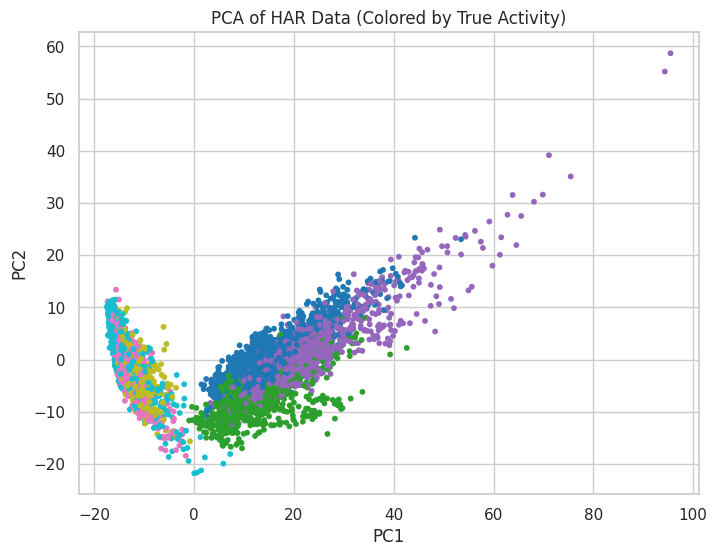
\includegraphics[width=0.8\linewidth]{expt-7_files/expt-7_5_0.png}
\end{center}

    
    \textbf{K-Means Clustering + Elbow/Sillhouette}

    \begin{tcolorbox}[breakable, size=fbox, boxrule=1pt, pad at break*=1mm,colback=cellbackground, colframe=cellborder]
\prompt{In}{incolor}{64}{\boxspacing}
\begin{Verbatim}[commandchars=\\\{\}]
\PY{n}{wcss} \PY{o}{=} \PY{p}{[}\PY{p}{]}
\PY{n}{sil\PYZus{}scores} \PY{o}{=} \PY{p}{[}\PY{p}{]}
\PY{n}{K\PYZus{}range} \PY{o}{=} \PY{n+nb}{range}\PY{p}{(}\PY{l+m+mi}{2}\PY{p}{,}\PY{l+m+mi}{9}\PY{p}{)}

\PY{k}{for} \PY{n}{k} \PY{o+ow}{in} \PY{n}{K\PYZus{}range}\PY{p}{:}
    \PY{n}{kmeans} \PY{o}{=} \PY{n}{KMeans}\PY{p}{(}\PY{n}{n\PYZus{}clusters}\PY{o}{=}\PY{n}{k}\PY{p}{,} \PY{n}{random\PYZus{}state}\PY{o}{=}\PY{l+m+mi}{42}\PY{p}{,} \PY{n}{n\PYZus{}init}\PY{o}{=}\PY{l+m+mi}{10}\PY{p}{)}
    \PY{n}{labels} \PY{o}{=} \PY{n}{kmeans}\PY{o}{.}\PY{n}{fit\PYZus{}predict}\PY{p}{(}\PY{n}{X\PYZus{}scaled}\PY{p}{)}
    \PY{n}{wcss}\PY{o}{.}\PY{n}{append}\PY{p}{(}\PY{n}{kmeans}\PY{o}{.}\PY{n}{inertia\PYZus{}}\PY{p}{)}
    \PY{n}{sil\PYZus{}scores}\PY{o}{.}\PY{n}{append}\PY{p}{(}\PY{n}{silhouette\PYZus{}score}\PY{p}{(}\PY{n}{X\PYZus{}scaled}\PY{p}{,} \PY{n}{labels}\PY{p}{)}\PY{p}{)}

\PY{n}{plt}\PY{o}{.}\PY{n}{figure}\PY{p}{(}\PY{n}{figsize}\PY{o}{=}\PY{p}{(}\PY{l+m+mi}{8}\PY{p}{,}\PY{l+m+mi}{4}\PY{p}{)}\PY{p}{)}
\PY{n}{plt}\PY{o}{.}\PY{n}{plot}\PY{p}{(}\PY{n}{K\PYZus{}range}\PY{p}{,} \PY{n}{wcss}\PY{p}{,} \PY{n}{marker}\PY{o}{=}\PY{l+s+s1}{\PYZsq{}}\PY{l+s+s1}{o}\PY{l+s+s1}{\PYZsq{}}\PY{p}{)}
\PY{n}{plt}\PY{o}{.}\PY{n}{xlabel}\PY{p}{(}\PY{l+s+s1}{\PYZsq{}}\PY{l+s+s1}{Number of clusters (k)}\PY{l+s+s1}{\PYZsq{}}\PY{p}{)}
\PY{n}{plt}\PY{o}{.}\PY{n}{ylabel}\PY{p}{(}\PY{l+s+s1}{\PYZsq{}}\PY{l+s+s1}{WCSS (Inertia)}\PY{l+s+s1}{\PYZsq{}}\PY{p}{)}
\PY{n}{plt}\PY{o}{.}\PY{n}{title}\PY{p}{(}\PY{l+s+s1}{\PYZsq{}}\PY{l+s+s1}{K\PYZhy{}Means Elbow Method}\PY{l+s+s1}{\PYZsq{}}\PY{p}{)}
\PY{n}{plt}\PY{o}{.}\PY{n}{show}\PY{p}{(}\PY{p}{)}
\end{Verbatim}
\end{tcolorbox}
    \begin{center}
    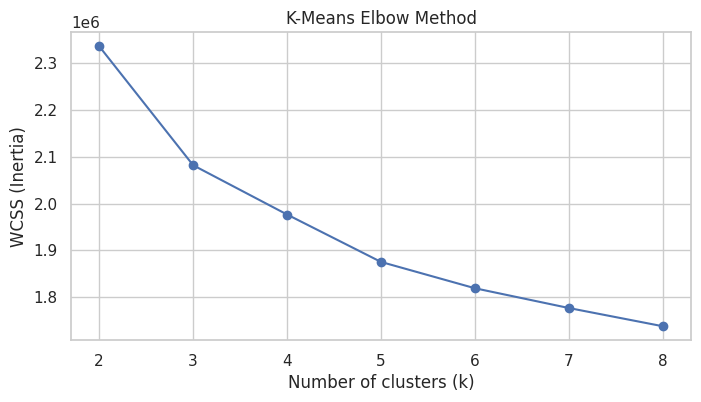
\includegraphics[width=0.8\linewidth]{expt-7_files/expt-7_7_0.png}
\end{center}
    
    \begin{tcolorbox}[breakable, size=fbox, boxrule=1pt, pad at break*=1mm,colback=cellbackground, colframe=cellborder]
\prompt{In}{incolor}{65}{\boxspacing}
\begin{Verbatim}[commandchars=\\\{\}]
\PY{c+c1}{\PYZsh{} Silhouette curve}
\PY{n}{plt}\PY{o}{.}\PY{n}{figure}\PY{p}{(}\PY{n}{figsize}\PY{o}{=}\PY{p}{(}\PY{l+m+mi}{8}\PY{p}{,}\PY{l+m+mi}{4}\PY{p}{)}\PY{p}{)}
\PY{n}{plt}\PY{o}{.}\PY{n}{plot}\PY{p}{(}\PY{n}{K\PYZus{}range}\PY{p}{,} \PY{n}{sil\PYZus{}scores}\PY{p}{,} \PY{n}{marker}\PY{o}{=}\PY{l+s+s1}{\PYZsq{}}\PY{l+s+s1}{o}\PY{l+s+s1}{\PYZsq{}}\PY{p}{,} \PY{n}{color}\PY{o}{=}\PY{l+s+s1}{\PYZsq{}}\PY{l+s+s1}{orange}\PY{l+s+s1}{\PYZsq{}}\PY{p}{)}
\PY{n}{plt}\PY{o}{.}\PY{n}{xlabel}\PY{p}{(}\PY{l+s+s1}{\PYZsq{}}\PY{l+s+s1}{Number of clusters (k)}\PY{l+s+s1}{\PYZsq{}}\PY{p}{)}
\PY{n}{plt}\PY{o}{.}\PY{n}{ylabel}\PY{p}{(}\PY{l+s+s1}{\PYZsq{}}\PY{l+s+s1}{Silhouette Score}\PY{l+s+s1}{\PYZsq{}}\PY{p}{)}
\PY{n}{plt}\PY{o}{.}\PY{n}{title}\PY{p}{(}\PY{l+s+s1}{\PYZsq{}}\PY{l+s+s1}{K\PYZhy{}Means Silhouette Score}\PY{l+s+s1}{\PYZsq{}}\PY{p}{)}
\PY{n}{plt}\PY{o}{.}\PY{n}{show}\PY{p}{(}\PY{p}{)}
\end{Verbatim}
\end{tcolorbox}

    \begin{center}
    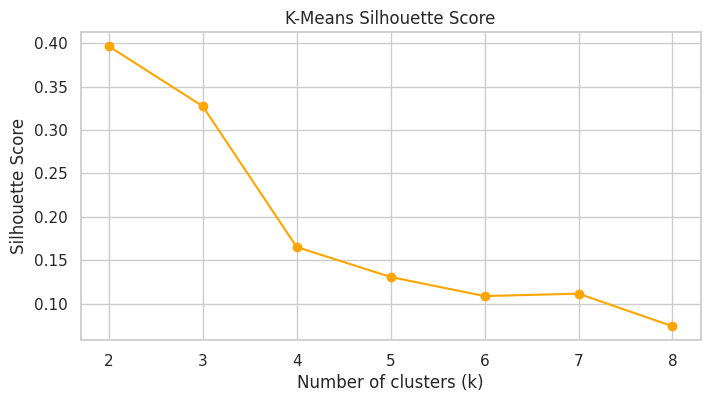
\includegraphics[width=0.8\linewidth]{expt-7_files/expt-7_8_0.png}
\end{center}
    
    \begin{tcolorbox}[breakable, size=fbox, boxrule=1pt, pad at break*=1mm,colback=cellbackground, colframe=cellborder]
\prompt{In}{incolor}{68}{\boxspacing}
\begin{Verbatim}[commandchars=\\\{\}]
\PY{n}{table} \PY{o}{=} \PY{n}{pd}\PY{o}{.}\PY{n}{DataFrame}\PY{p}{(}\PY{p}{\PYZob{}}
        \PY{l+s+s2}{\PYZdq{}}\PY{l+s+s2}{k}\PY{l+s+s2}{\PYZdq{}}\PY{p}{:} \PY{n+nb}{list}\PY{p}{(}\PY{n}{K\PYZus{}range}\PY{p}{)}\PY{p}{,}
        \PY{l+s+s2}{\PYZdq{}}\PY{l+s+s2}{WCSS}\PY{l+s+s2}{\PYZdq{}}\PY{p}{:} \PY{n}{wcss}\PY{p}{,}
        \PY{l+s+s2}{\PYZdq{}}\PY{l+s+s2}{Silhouette}\PY{l+s+s2}{\PYZdq{}}\PY{p}{:} \PY{n}{sil\PYZus{}scores}
    \PY{p}{\PYZcb{}}\PY{p}{)}
\PY{n+nb}{print}\PY{p}{(}\PY{n}{table}\PY{o}{.}\PY{n}{to\PYZus{}string}\PY{p}{(}\PY{n}{index}\PY{o}{=}\PY{k+kc}{False}\PY{p}{)}\PY{p}{)}
\end{Verbatim}
\end{tcolorbox}

    \begin{Verbatim}[commandchars=\\\{\}]
 k         WCSS  Silhouette
 2 2.336224e+06    0.396505
 3 2.081850e+06    0.327408
 4 1.976453e+06    0.165163
 5 1.875066e+06    0.130639
 6 1.818790e+06    0.108641
 7 1.776519e+06    0.111424
 8 1.737555e+06    0.073861
    \end{Verbatim}

    \begin{tcolorbox}[breakable, size=fbox, boxrule=1pt, pad at break*=1mm,colback=cellbackground, colframe=cellborder]
\prompt{In}{incolor}{80}{\boxspacing}
\begin{Verbatim}[commandchars=\\\{\}]
\PY{c+c1}{\PYZsh{} choosing best k}
\PY{n}{k\PYZus{}best} \PY{o}{=} \PY{l+m+mi}{3}
\PY{n}{kmeans} \PY{o}{=} \PY{n}{KMeans}\PY{p}{(}\PY{n}{n\PYZus{}clusters}\PY{o}{=}\PY{n}{k\PYZus{}best}\PY{p}{,} \PY{n}{random\PYZus{}state}\PY{o}{=}\PY{l+m+mi}{42}\PY{p}{,} \PY{n}{n\PYZus{}init}\PY{o}{=}\PY{l+m+mi}{10}\PY{p}{)}
\PY{n}{k\PYZus{}labels} \PY{o}{=} \PY{n}{kmeans}\PY{o}{.}\PY{n}{fit\PYZus{}predict}\PY{p}{(}\PY{n}{X\PYZus{}scaled}\PY{p}{)}
\end{Verbatim}
\end{tcolorbox}

    \begin{tcolorbox}[breakable, size=fbox, boxrule=1pt, pad at break*=1mm,colback=cellbackground, colframe=cellborder]
\prompt{In}{incolor}{81}{\boxspacing}
\begin{Verbatim}[commandchars=\\\{\}]
\PY{c+c1}{\PYZsh{} PCA visualization of clusters}
\PY{n}{plt}\PY{o}{.}\PY{n}{figure}\PY{p}{(}\PY{n}{figsize}\PY{o}{=}\PY{p}{(}\PY{l+m+mi}{8}\PY{p}{,}\PY{l+m+mi}{6}\PY{p}{)}\PY{p}{)}
\PY{n}{plt}\PY{o}{.}\PY{n}{scatter}\PY{p}{(}\PY{n}{X\PYZus{}pca}\PY{p}{[}\PY{p}{:}\PY{p}{,}\PY{l+m+mi}{0}\PY{p}{]}\PY{p}{,} \PY{n}{X\PYZus{}pca}\PY{p}{[}\PY{p}{:}\PY{p}{,}\PY{l+m+mi}{1}\PY{p}{]}\PY{p}{,} \PY{n}{c}\PY{o}{=}\PY{n}{k\PYZus{}labels}\PY{p}{,} \PY{n}{cmap}\PY{o}{=}\PY{l+s+s1}{\PYZsq{}}\PY{l+s+s1}{tab10}\PY{l+s+s1}{\PYZsq{}}\PY{p}{,} \PY{n}{s}\PY{o}{=}\PY{l+m+mi}{10}\PY{p}{)}
\PY{n}{plt}\PY{o}{.}\PY{n}{title}\PY{p}{(}\PY{l+s+sa}{f}\PY{l+s+s1}{\PYZsq{}}\PY{l+s+s1}{K\PYZhy{}Means Clusters (k=}\PY{l+s+si}{\PYZob{}}\PY{n}{k\PYZus{}best}\PY{l+s+si}{\PYZcb{}}\PY{l+s+s1}{)}\PY{l+s+s1}{\PYZsq{}}\PY{p}{)}
\PY{n}{plt}\PY{o}{.}\PY{n}{xlabel}\PY{p}{(}\PY{l+s+s1}{\PYZsq{}}\PY{l+s+s1}{PC1}\PY{l+s+s1}{\PYZsq{}}\PY{p}{)}\PY{p}{;} \PY{n}{plt}\PY{o}{.}\PY{n}{ylabel}\PY{p}{(}\PY{l+s+s1}{\PYZsq{}}\PY{l+s+s1}{PC2}\PY{l+s+s1}{\PYZsq{}}\PY{p}{)}
\PY{n}{plt}\PY{o}{.}\PY{n}{show}\PY{p}{(}\PY{p}{)}
\end{Verbatim}
\end{tcolorbox}

    \begin{center}
    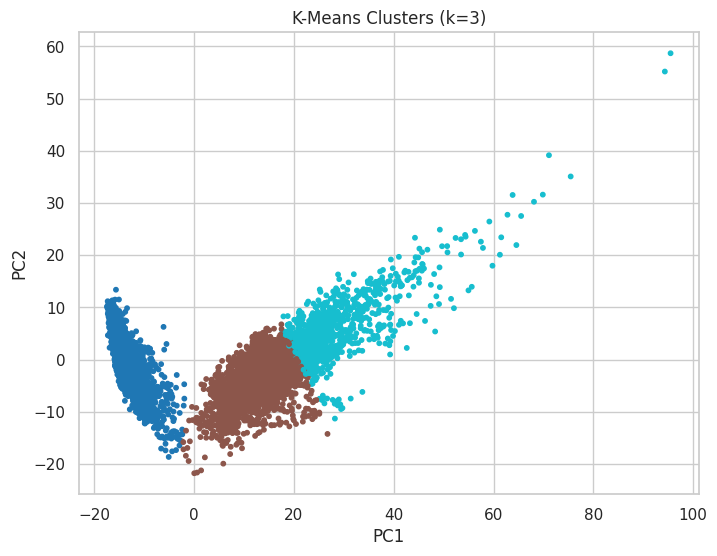
\includegraphics[width=0.8\linewidth]{expt-7_files/expt-7_11_0.png}
\end{center}
    
    \begin{tcolorbox}[breakable, size=fbox, boxrule=1pt, pad at break*=1mm,colback=cellbackground, colframe=cellborder]
\prompt{In}{incolor}{105}{\boxspacing}
\begin{Verbatim}[commandchars=\\\{\}]
\PY{k}{def}\PY{+w}{ }\PY{n+nf}{cluster\PYZus{}confusion\PYZus{}matrix}\PY{p}{(}\PY{n}{true\PYZus{}labels}\PY{p}{,} \PY{n}{cluster\PYZus{}labels}\PY{p}{,} \PY{n}{algo\PYZus{}name}\PY{o}{=}\PY{l+s+s2}{\PYZdq{}}\PY{l+s+s2}{K\PYZhy{}Means}\PY{l+s+s2}{\PYZdq{}}\PY{p}{)}\PY{p}{:}
    \PY{c+c1}{\PYZsh{} Map clusters to most common true label}
    \PY{n}{labels} \PY{o}{=} \PY{n}{np}\PY{o}{.}\PY{n}{unique}\PY{p}{(}\PY{n}{cluster\PYZus{}labels}\PY{p}{)}
    \PY{n}{mapping} \PY{o}{=} \PY{p}{\PYZob{}}\PY{p}{\PYZcb{}}
    \PY{k}{for} \PY{n}{lbl} \PY{o+ow}{in} \PY{n}{labels}\PY{p}{:}
        \PY{n}{mask} \PY{o}{=} \PY{n}{cluster\PYZus{}labels} \PY{o}{==} \PY{n}{lbl}
        \PY{n}{true\PYZus{}for\PYZus{}cluster} \PY{o}{=} \PY{n}{true\PYZus{}labels}\PY{p}{[}\PY{n}{mask}\PY{p}{]}
        \PY{k}{if} \PY{n+nb}{len}\PY{p}{(}\PY{n}{true\PYZus{}for\PYZus{}cluster}\PY{p}{)} \PY{o}{==} \PY{l+m+mi}{0}\PY{p}{: continue}
        \PY{n}{mapping}\PY{p}{[}\PY{n}{lbl}\PY{p}{]} \PY{o}{=} \PY{n}{np}\PY{o}{.}\PY{n}{bincount}\PY{p}{(}\PY{n}{true\PYZus{}for\PYZus{}cluster}\PY{p}{)}\PY{o}{.}\PY{n}{argmax}\PY{p}{(}\PY{p}{)}

    \PY{n}{mapped\PYZus{}labels} \PY{o}{=} \PY{n}{np}\PY{o}{.}\PY{n}{array}\PY{p}{(}\PY{p}{[}\PY{n}{mapping}\PY{p}{[}\PY{n}{lbl}\PY{p}{]} \PY{k}{for} \PY{n}{lbl} \PY{o+ow}{in} \PY{n}{cluster\PYZus{}labels}\PY{p}{]}\PY{p}{)}

    \PY{c+c1}{\PYZsh{} Compute confusion matrix}
    \PY{n}{cm} \PY{o}{=} \PY{n}{confusion\PYZus{}matrix}\PY{p}{(}\PY{n}{true\PYZus{}labels}\PY{p}{,} \PY{n}{mapped\PYZus{}labels}\PY{p}{)}
    \PY{n}{cm\PYZus{}df} \PY{o}{=} \PY{n}{pd}\PY{o}{.}\PY{n}{DataFrame}\PY{p}{(}\PY{n}{cm}\PY{p}{,} \PY{n}{index}\PY{o}{=}\PY{n}{np}\PY{o}{.}\PY{n}{unique}\PY{p}{(}\PY{n}{true\PYZus{}labels}\PY{p}{)}\PY{p}{,} \PY{n}{columns}\PY{o}{=}\PY{n}{np}\PY{o}{.}\PY{n}{unique}\PY{p}{(}\PY{n}{true\PYZus{}labels}\PY{p}{)}\PY{p}{)}

    \PY{n}{plt}\PY{o}{.}\PY{n}{figure}\PY{p}{(}\PY{n}{figsize}\PY{o}{=}\PY{p}{(}\PY{l+m+mi}{6}\PY{p}{,}\PY{l+m+mi}{5}\PY{p}{)}\PY{p}{)}
    \PY{n}{sns}\PY{o}{.}\PY{n}{heatmap}\PY{p}{(}\PY{n}{cm\PYZus{}df}\PY{p}{,} \PY{n}{annot}\PY{o}{=}\PY{k+kc}{True}\PY{p}{,} \PY{n}{fmt}\PY{o}{=}\PY{l+s+s2}{\PYZdq{}}\PY{l+s+s2}{d}\PY{l+s+s2}{\PYZdq{}}\PY{p}{,} \PY{n}{cmap}\PY{o}{=}\PY{l+s+s2}{\PYZdq{}}\PY{l+s+s2}{Blues}\PY{l+s+s2}{\PYZdq{}}\PY{p}{)}
    \PY{n}{plt}\PY{o}{.}\PY{n}{title}\PY{p}{(}\PY{l+s+sa}{f}\PY{l+s+s2}{\PYZdq{}}\PY{l+s+si}{\PYZob{}}\PY{n}{algo\PYZus{}name}\PY{l+s+si}{\PYZcb{}}\PY{l+s+s2}{ Confusion Matrix}\PY{l+s+s2}{\PYZdq{}}\PY{p}{)}
    \PY{n}{plt}\PY{o}{.}\PY{n}{xlabel}\PY{p}{(}\PY{l+s+s2}{\PYZdq{}}\PY{l+s+s2}{Predicted (Cluster\PYZhy{}mapped)}\PY{l+s+s2}{\PYZdq{}}\PY{p}{)}
    \PY{n}{plt}\PY{o}{.}\PY{n}{ylabel}\PY{p}{(}\PY{l+s+s2}{\PYZdq{}}\PY{l+s+s2}{True Activity}\PY{l+s+s2}{\PYZdq{}}\PY{p}{)}
    \PY{n}{plt}\PY{o}{.}\PY{n}{show}\PY{p}{(}\PY{p}{)}
    \PY{k}{return} \PY{n}{cm\PYZus{}df}

\PY{n}{cm\PYZus{}kmeans} \PY{o}{=} \PY{n}{cluster\PYZus{}confusion\PYZus{}matrix}\PY{p}{(}\PY{n}{y\PYZus{}train}\PY{p}{[}\PY{l+m+mi}{0}\PY{p}{]}\PY{o}{.}\PY{n}{values}\PY{p}{,} \PY{n}{k\PYZus{}labels}\PY{p}{,} \PY{l+s+s2}{\PYZdq{}}\PY{l+s+s2}{K\PYZhy{}Means}\PY{l+s+s2}{\PYZdq{}}\PY{p}{)}
\end{Verbatim}
\end{tcolorbox}
    \begin{center}
    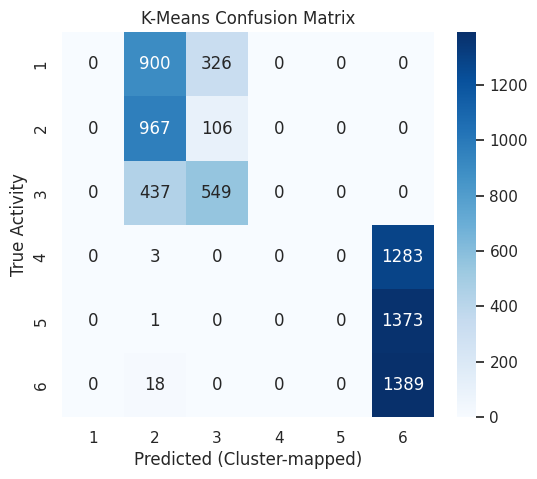
\includegraphics[width=0.8\linewidth]{expt-7_files/expt-7_12_0.png}
\end{center}
    
    \textbf{DBScan}

    \begin{tcolorbox}[breakable, size=fbox, boxrule=1pt, pad at break*=1mm,colback=cellbackground, colframe=cellborder]
\prompt{In}{incolor}{88}{\boxspacing}
\begin{Verbatim}[commandchars=\\\{\}]
\PY{k}{def}\PY{+w}{ }\PY{n+nf}{tune\PYZus{}dbscan}\PY{p}{(}\PY{n}{X}\PY{p}{,} \PY{n}{eps\PYZus{}values}\PY{p}{,} \PY{n}{min\PYZus{}samples\PYZus{}values}\PY{p}{)}\PY{p}{:}
    \PY{n}{best\PYZus{}score} \PY{o}{=} \PY{o}{\PYZhy{}}\PY{l+m+mi}{1}
    \PY{n}{best\PYZus{}params} \PY{o}{=} \PY{k+kc}{None}
    \PY{n}{results} \PY{o}{=} \PY{p}{[}\PY{p}{]}

    \PY{k}{for} \PY{n}{eps} \PY{o+ow}{in} \PY{n}{eps\PYZus{}values}\PY{p}{:}
        \PY{k}{for} \PY{n}{min\PYZus{}s} \PY{o+ow}{in} \PY{n}{min\PYZus{}samples\PYZus{}values}\PY{p}{:}
            \PY{n}{db} \PY{o}{=} \PY{n}{DBSCAN}\PY{p}{(}\PY{n}{eps}\PY{o}{=}\PY{n}{eps}\PY{p}{,} \PY{n}{min\PYZus{}samples}\PY{o}{=}\PY{n}{min\PYZus{}s}\PY{p}{)}\PY{o}{.}\PY{n}{fit}\PY{p}{(}\PY{n}{X}\PY{p}{)}
            \PY{n}{labels} \PY{o}{=} \PY{n}{db}\PY{o}{.}\PY{n}{labels\PYZus{}}

            \PY{c+c1}{\PYZsh{} skip if DBSCAN assigns all points to noise or 1 cluster}
            \PY{k}{if} \PY{n+nb}{len}\PY{p}{(}\PY{n+nb}{set}\PY{p}{(}\PY{n}{labels}\PY{p}{)}\PY{p}{)} \PY{o}{\PYZlt{}}\PY{o}{=} \PY{l+m+mi}{1}\PY{p}{:}
                \PY{k}{continue}

            \PY{k}{try}\PY{p}{:}
                \PY{n}{sil} \PY{o}{=} \PY{n}{silhouette\PYZus{}score}\PY{p}{(}\PY{n}{X}\PY{p}{,} \PY{n}{labels}\PY{p}{)}
                \PY{n}{dbi} \PY{o}{=} \PY{n}{davies\PYZus{}bouldin\PYZus{}score}\PY{p}{(}\PY{n}{X}\PY{p}{,} \PY{n}{labels}\PY{p}{)}
                \PY{n}{ch} \PY{o}{=} \PY{n}{calinski\PYZus{}harabasz\PYZus{}score}\PY{p}{(}\PY{n}{X}\PY{p}{,} \PY{n}{labels}\PY{p}{)}
            \PY{k}{except}\PY{p}{:}
                \PY{k}{continue}

            \PY{n}{results}\PY{o}{.}\PY{n}{append}\PY{p}{(}\PY{p}{(}\PY{n}{eps}\PY{p}{,} \PY{n}{min\PYZus{}s}\PY{p}{,} \PY{n}{sil}\PY{p}{,} \PY{n}{dbi}\PY{p}{,} \PY{n}{ch}\PY{p}{)}\PY{p}{)}

            \PY{k}{if} \PY{n}{sil} \PY{o}{\PYZgt{}} \PY{n}{best\PYZus{}score}\PY{p}{:}
                \PY{n}{best\PYZus{}score} \PY{o}{=} \PY{n}{sil}
                \PY{n}{best\PYZus{}params} \PY{o}{=} \PY{p}{(}\PY{n}{eps}\PY{p}{,} \PY{n}{min\PYZus{}s}\PY{p}{)}

    \PY{k}{return} \PY{n}{best\PYZus{}params}\PY{p}{,} \PY{n}{results}

\PY{c+c1}{\PYZsh{} Example usage}
\PY{n}{eps\PYZus{}range} \PY{o}{=} \PY{n}{np}\PY{o}{.}\PY{n}{linspace}\PY{p}{(}\PY{l+m+mi}{10}\PY{p}{,} \PY{l+m+mi}{15}\PY{p}{,} \PY{l+m+mi}{20}\PY{p}{,} \PY{l+m+mi}{25}\PY{p}{)}
\PY{n}{min\PYZus{}samples\PYZus{}range} \PY{o}{=} \PY{p}{[}\PY{l+m+mi}{5}\PY{p}{,} \PY{l+m+mi}{10}\PY{p}{,} \PY{l+m+mi}{15}\PY{p}{,} \PY{l+m+mi}{20}\PY{p}{]}

\PY{n}{best\PYZus{}params}\PY{p}{,} \PY{n}{results} \PY{o}{=} \PY{n}{tune\PYZus{}dbscan}\PY{p}{(}\PY{n}{X\PYZus{}scaled}\PY{p}{,} \PY{n}{eps\PYZus{}range}\PY{p}{,} \PY{n}{min\PYZus{}samples\PYZus{}range}\PY{p}{)}

\PY{k}{if} \PY{n}{best\PYZus{}params} \PY{o+ow}{is} \PY{k+kc}{None}\PY{p}{:}
    \PY{n+nb}{print}\PY{p}{(}\PY{l+s+s2}{\PYZdq{}}\PY{l+s+s2}{DBSCAN couldn}\PY{l+s+s2}{\PYZsq{}}\PY{l+s+s2}{t form valid clusters in the tested range.}\PY{l+s+s2}{\PYZdq{}}\PY{p}{)}
\PY{k}{else}\PY{p}{:}
    \PY{n+nb}{print}\PY{p}{(}\PY{l+s+s2}{\PYZdq{}}\PY{l+s+s2}{Best params:}\PY{l+s+s2}{\PYZdq{}}\PY{p}{,} \PY{n}{best\PYZus{}params}\PY{p}{)}
    
\end{Verbatim}
\end{tcolorbox}

    \begin{Verbatim}[commandchars=\\\{\}]
    
Best params: (np.float64(14.0), 20)

    \end{Verbatim}

    \begin{tcolorbox}[breakable, size=fbox, boxrule=1pt, pad at break*=1mm,colback=cellbackground, colframe=cellborder]
\prompt{In}{incolor}{91}{\boxspacing}
\begin{Verbatim}[commandchars=\\\{\}]
\PY{n}{dbscan} \PY{o}{=} \PY{n}{DBSCAN}\PY{p}{(}\PY{n}{eps}\PY{o}{=}\PY{l+m+mi}{14}\PY{p}{,} \PY{n}{min\PYZus{}samples}\PY{o}{=}\PY{l+m+mi}{20}\PY{p}{)}
\PY{n}{db\PYZus{}labels} \PY{o}{=} \PY{n}{dbscan}\PY{o}{.}\PY{n}{fit\PYZus{}predict}\PY{p}{(}\PY{n}{X\PYZus{}scaled}\PY{p}{)}

\PY{n}{plt}\PY{o}{.}\PY{n}{figure}\PY{p}{(}\PY{n}{figsize}\PY{o}{=}\PY{p}{(}\PY{l+m+mi}{8}\PY{p}{,}\PY{l+m+mi}{6}\PY{p}{)}\PY{p}{)}
\PY{n}{plt}\PY{o}{.}\PY{n}{scatter}\PY{p}{(}\PY{n}{X\PYZus{}pca}\PY{p}{[}\PY{p}{:}\PY{p}{,}\PY{l+m+mi}{0}\PY{p}{]}\PY{p}{,} \PY{n}{X\PYZus{}pca}\PY{p}{[}\PY{p}{:}\PY{p}{,}\PY{l+m+mi}{1}\PY{p}{]}\PY{p}{,} \PY{n}{c}\PY{o}{=}\PY{n}{db\PYZus{}labels}\PY{p}{,} \PY{n}{cmap}\PY{o}{=}\PY{l+s+s1}{\PYZsq{}}\PY{l+s+s1}{tab10}\PY{l+s+s1}{\PYZsq{}}\PY{p}{,} \PY{n}{s}\PY{o}{=}\PY{l+m+mi}{10}\PY{p}{)}
\PY{n}{plt}\PY{o}{.}\PY{n}{title}\PY{p}{(}\PY{l+s+s1}{\PYZsq{}}\PY{l+s+s1}{DBSCAN Clusters}\PY{l+s+s1}{\PYZsq{}}\PY{p}{)}
\PY{n}{plt}\PY{o}{.}\PY{n}{xlabel}\PY{p}{(}\PY{l+s+s1}{\PYZsq{}}\PY{l+s+s1}{PC1}\PY{l+s+s1}{\PYZsq{}}\PY{p}{)}\PY{p}{;} \PY{n}{plt}\PY{o}{.}\PY{n}{ylabel}\PY{p}{(}\PY{l+s+s1}{\PYZsq{}}\PY{l+s+s1}{PC2}\PY{l+s+s1}{\PYZsq{}}\PY{p}{)}
\PY{n}{plt}\PY{o}{.}\PY{n}{show}\PY{p}{(}\PY{p}{)}

\end{Verbatim}
\end{tcolorbox}

    \begin{center}
    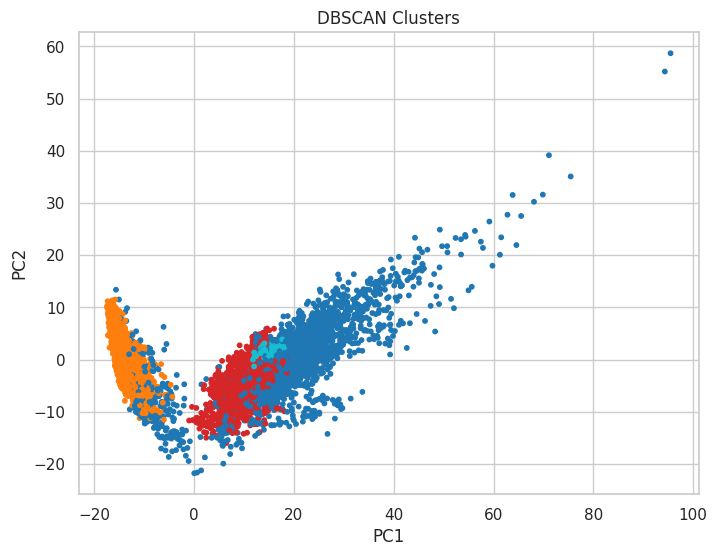
\includegraphics[width=0.9\linewidth]{expt-7_files/expt-7_15_0.png}
\end{center}
    
    \textbf{Hierarchical Clustering}

    \begin{tcolorbox}[breakable, size=fbox, boxrule=1pt, pad at break*=1mm,colback=cellbackground, colframe=cellborder]
\prompt{In}{incolor}{83}{\boxspacing}
\begin{Verbatim}[commandchars=\\\{\}]

\PY{n}{agg} \PY{o}{=} \PY{n}{AgglomerativeClustering}\PY{p}{(}\PY{n}{n\PYZus{}clusters}\PY{o}{=}\PY{n}{k\PYZus{}best}\PY{p}{,} \PY{n}{linkage}\PY{o}{=}\PY{l+s+s1}{\PYZsq{}}\PY{l+s+s1}{ward}\PY{l+s+s1}{\PYZsq{}}\PY{p}{)}
\PY{n}{agg\PYZus{}labels} \PY{o}{=} \PY{n}{agg}\PY{o}{.}\PY{n}{fit\PYZus{}predict}\PY{p}{(}\PY{n}{X\PYZus{}scaled}\PY{p}{)}

\PY{n}{plt}\PY{o}{.}\PY{n}{figure}\PY{p}{(}\PY{n}{figsize}\PY{o}{=}\PY{p}{(}\PY{l+m+mi}{8}\PY{p}{,}\PY{l+m+mi}{6}\PY{p}{)}\PY{p}{)}
\PY{n}{plt}\PY{o}{.}\PY{n}{scatter}\PY{p}{(}\PY{n}{X\PYZus{}pca}\PY{p}{[}\PY{p}{:}\PY{p}{,}\PY{l+m+mi}{0}\PY{p}{]}\PY{p}{,} \PY{n}{X\PYZus{}pca}\PY{p}{[}\PY{p}{:}\PY{p}{,}\PY{l+m+mi}{1}\PY{p}{]}\PY{p}{,} \PY{n}{c}\PY{o}{=}\PY{n}{agg\PYZus{}labels}\PY{p}{,} \PY{n}{cmap}\PY{o}{=}\PY{l+s+s1}{\PYZsq{}}\PY{l+s+s1}{tab10}\PY{l+s+s1}{\PYZsq{}}\PY{p}{,} \PY{n}{s}\PY{o}{=}\PY{l+m+mi}{10}\PY{p}{)}
\PY{n}{plt}\PY{o}{.}\PY{n}{title}\PY{p}{(}\PY{l+s+s1}{\PYZsq{}}\PY{l+s+s1}{Hierarchical Clustering (Ward)}\PY{l+s+s1}{\PYZsq{}}\PY{p}{)}
\PY{n}{plt}\PY{o}{.}\PY{n}{xlabel}\PY{p}{(}\PY{l+s+s1}{\PYZsq{}}\PY{l+s+s1}{PC1}\PY{l+s+s1}{\PYZsq{}}\PY{p}{)}\PY{p}{;} \PY{n}{plt}\PY{o}{.}\PY{n}{ylabel}\PY{p}{(}\PY{l+s+s1}{\PYZsq{}}\PY{l+s+s1}{PC2}\PY{l+s+s1}{\PYZsq{}}\PY{p}{)}
\PY{n}{plt}\PY{o}{.}\PY{n}{show}\PY{p}{(}\PY{p}{)}

\end{Verbatim}
\end{tcolorbox}
    \begin{center}
    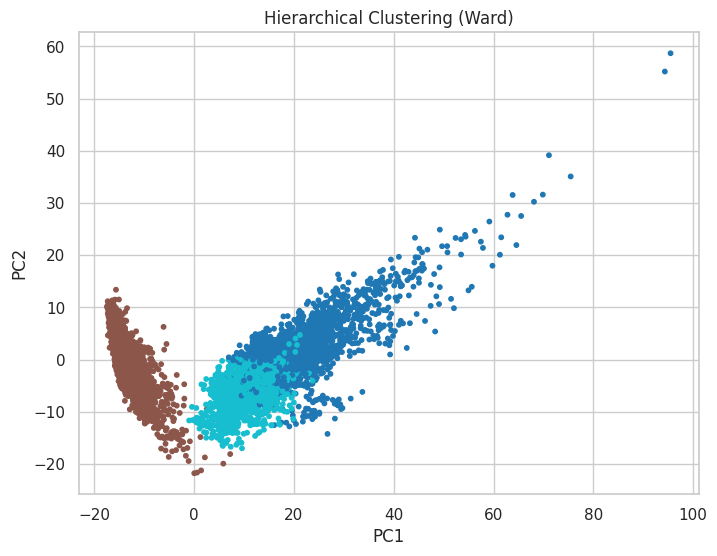
\includegraphics[width=0.9\linewidth]{expt-7_files/expt-7_17_0.png}
\end{center}
    
    \begin{tcolorbox}[breakable, size=fbox, boxrule=1pt, pad at break*=1mm,colback=cellbackground, colframe=cellborder]
\prompt{In}{incolor}{93}{\boxspacing}
\begin{Verbatim}[commandchars=\\\{\}]

\PY{k+kn}{from}\PY{+w}{ }\PY{n+nn}{scipy}\PY{n+nn}{.}\PY{n+nn}{cluster}\PY{n+nn}{.}\PY{n+nn}{hierarchy}\PY{+w}{ }\PY{k+kn}{import} \PY{n}{dendrogram}\PY{p}{,} \PY{n}{linkage}
\PY{k+kn}{import}\PY{+w}{ }\PY{n+nn}{matplotlib}\PY{n+nn}{.}\PY{n+nn}{pyplot}\PY{+w}{ }\PY{k}{as}\PY{+w}{ }\PY{n+nn}{plt}

\PY{c+c1}{\PYZsh{} Using Ward linkage}
\PY{n}{Z} \PY{o}{=} \PY{n}{linkage}\PY{p}{(}\PY{n}{X\PYZus{}scaled}\PY{p}{,} \PY{n}{method}\PY{o}{=}\PY{l+s+s1}{\PYZsq{}}\PY{l+s+s1}{ward}\PY{l+s+s1}{\PYZsq{}}\PY{p}{)}

\PY{n}{plt}\PY{o}{.}\PY{n}{figure}\PY{p}{(}\PY{n}{figsize}\PY{o}{=}\PY{p}{(}\PY{l+m+mi}{12}\PY{p}{,}\PY{l+m+mi}{6}\PY{p}{)}\PY{p}{)}
\PY{n}{dendrogram}\PY{p}{(}\PY{n}{Z}\PY{p}{,} \PY{n}{truncate\PYZus{}mode}\PY{o}{=}\PY{l+s+s1}{\PYZsq{}}\PY{l+s+s1}{level}\PY{l+s+s1}{\PYZsq{}}\PY{p}{,} \PY{n}{p}\PY{o}{=}\PY{l+m+mi}{5}\PY{p}{,} \PY{n}{leaf\PYZus{}rotation}\PY{o}{=}\PY{l+m+mi}{90}\PY{p}{,} \PY{n}{leaf\PYZus{}font\PYZus{}size}\PY{o}{=}\PY{l+m+mi}{10}\PY{p}{)}
\PY{n}{plt}\PY{o}{.}\PY{n}{title}\PY{p}{(}\PY{l+s+s2}{\PYZdq{}}\PY{l+s+s2}{Hierarchical Clustering Dendrogram (truncated)}\PY{l+s+s2}{\PYZdq{}}\PY{p}{)}
\PY{n}{plt}\PY{o}{.}\PY{n}{xlabel}\PY{p}{(}\PY{l+s+s2}{\PYZdq{}}\PY{l+s+s2}{Samples / Index}\PY{l+s+s2}{\PYZdq{}}\PY{p}{)}
\PY{n}{plt}\PY{o}{.}\PY{n}{ylabel}\PY{p}{(}\PY{l+s+s2}{\PYZdq{}}\PY{l+s+s2}{Distance}\PY{l+s+s2}{\PYZdq{}}\PY{p}{)}
\PY{n}{plt}\PY{o}{.}\PY{n}{show}\PY{p}{(}\PY{p}{)}

\end{Verbatim}
\end{tcolorbox}

    \begin{center}
    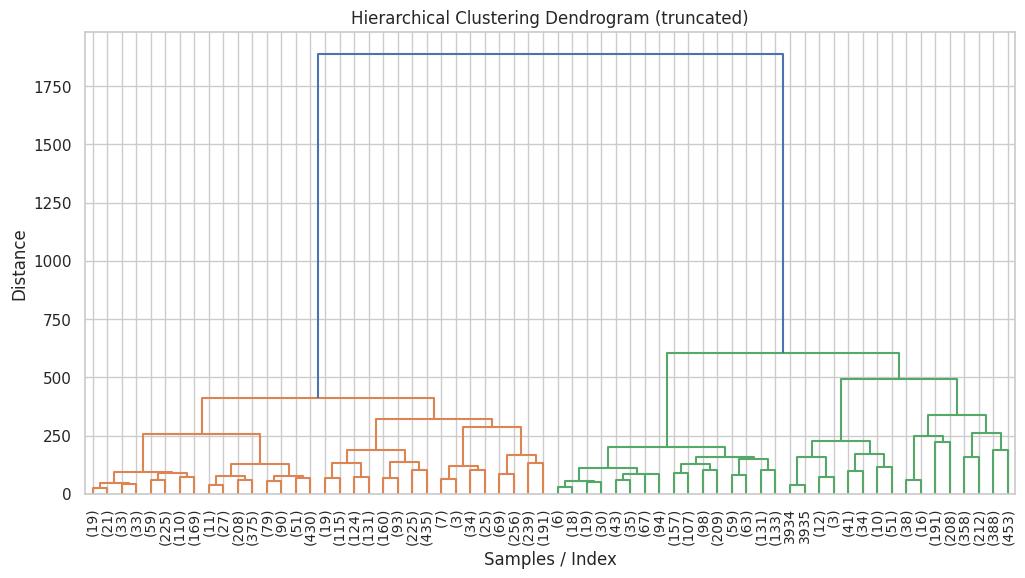
\includegraphics[width=0.9\linewidth]{expt-7_files/expt-7_18_0.png}
\end{center}
    
    \begin{tcolorbox}[breakable, size=fbox, boxrule=1pt, pad at break*=1mm,colback=cellbackground, colframe=cellborder]
\prompt{In}{incolor}{92}{\boxspacing}
\begin{Verbatim}[commandchars=\\\{\}]
\PY{c+c1}{\PYZsh{} EVALUATION METRICES}
\PY{k}{def}\PY{+w}{ }\PY{n+nf}{clustering\PYZus{}metrics}\PY{p}{(}\PY{n}{X}\PY{p}{,} \PY{n}{cluster\PYZus{}labels}\PY{p}{,} \PY{n}{true\PYZus{}labels}\PY{o}{=}\PY{k+kc}{None}\PY{p}{,} \PY{n}{algo\PYZus{}name}\PY{o}{=}\PY{l+s+s2}{\PYZdq{}}\PY{l+s+s2}{Algorithm}\PY{l+s+s2}{\PYZdq{}}\PY{p}{)}\PY{p}{:}
    \PY{n}{metrics} \PY{o}{=} \PY{p}{\PYZob{}}\PY{p}{\PYZcb{}}
    \PY{n}{n\PYZus{}clusters} \PY{o}{=} \PY{n+nb}{len}\PY{p}{(}\PY{n+nb}{set}\PY{p}{(}\PY{n}{cluster\PYZus{}labels}\PY{p}{)}\PY{p}{)} \PY{o}{\PYZhy{}} \PY{p}{(}\PY{l+m+mi}{1} \PY{k}{if} \PY{o}{\PYZhy{}}\PY{l+m+mi}{1} \PY{o+ow}{in} \PY{n}{cluster\PYZus{}labels} \PY{k}{else} \PY{l+m+mi}{0}\PY{p}{)}  

    \PY{c+c1}{\PYZsh{} Internal metrics (if at least 2 clusters)}
    \PY{k}{if} \PY{n}{n\PYZus{}clusters} \PY{o}{\PYZgt{}} \PY{l+m+mi}{1}\PY{p}{:}
        \PY{n}{metrics}\PY{p}{[}\PY{l+s+s1}{\PYZsq{}}\PY{l+s+s1}{Silhouette}\PY{l+s+s1}{\PYZsq{}}\PY{p}{]} \PY{o}{=} \PY{n}{silhouette\PYZus{}score}\PY{p}{(}\PY{n}{X}\PY{p}{,} \PY{n}{cluster\PYZus{}labels}\PY{p}{)}
        \PY{n}{metrics}\PY{p}{[}\PY{l+s+s1}{\PYZsq{}}\PY{l+s+s1}{Davies\PYZhy{}Bouldin}\PY{l+s+s1}{\PYZsq{}}\PY{p}{]} \PY{o}{=} \PY{n}{davies\PYZus{}bouldin\PYZus{}score}\PY{p}{(}\PY{n}{X}\PY{p}{,} \PY{n}{cluster\PYZus{}labels}\PY{p}{)}
        \PY{n}{metrics}\PY{p}{[}\PY{l+s+s1}{\PYZsq{}}\PY{l+s+s1}{Calinski\PYZhy{}Harabasz}\PY{l+s+s1}{\PYZsq{}}\PY{p}{]} \PY{o}{=} \PY{n}{calinski\PYZus{}harabasz\PYZus{}score}\PY{p}{(}\PY{n}{X}\PY{p}{,} \PY{n}{cluster\PYZus{}labels}\PY{p}{)}

    \PY{c+c1}{\PYZsh{} External metrics (if true labels provided)}
    \PY{k}{if} \PY{n}{true\PYZus{}labels} \PY{o+ow}{is} \PY{o+ow}{not} \PY{k+kc}{None}\PY{p}{:}
        \PY{n}{metrics}\PY{p}{[}\PY{l+s+s1}{\PYZsq{}}\PY{l+s+s1}{ARI}\PY{l+s+s1}{\PYZsq{}}\PY{p}{]} \PY{o}{=} \PY{n}{adjusted\PYZus{}rand\PYZus{}score}\PY{p}{(}\PY{n}{true\PYZus{}labels}\PY{p}{,} \PY{n}{cluster\PYZus{}labels}\PY{p}{)}
        \PY{n}{metrics}\PY{p}{[}\PY{l+s+s1}{\PYZsq{}}\PY{l+s+s1}{NMI}\PY{l+s+s1}{\PYZsq{}}\PY{p}{]} \PY{o}{=} \PY{n}{normalized\PYZus{}mutual\PYZus{}info\PYZus{}score}\PY{p}{(}\PY{n}{true\PYZus{}labels}\PY{p}{,} \PY{n}{cluster\PYZus{}labels}\PY{p}{)}
        
    \PY{k}{return} \PY{n}{pd}\PY{o}{.}\PY{n}{DataFrame}\PY{p}{(}\PY{p}{\PYZob{}}\PY{n}{algo\PYZus{}name}\PY{p}{:} \PY{n}{metrics}\PY{p}{\PYZcb{}}\PY{p}{)}\PY{o}{.}\PY{n}{T}

\PY{n}{y\PYZus{}true} \PY{o}{=} \PY{n}{y\PYZus{}train}\PY{p}{[}\PY{l+m+mi}{0}\PY{p}{]}  \PY{c+c1}{\PYZsh{} ground truth}
\PY{n}{k\PYZus{}metrics} \PY{o}{=} \PY{n}{clustering\PYZus{}metrics}\PY{p}{(}\PY{n}{X\PYZus{}scaled}\PY{p}{,} \PY{n}{k\PYZus{}labels}\PY{p}{,} \PY{n}{y\PYZus{}true}\PY{p}{,} \PY{l+s+s2}{\PYZdq{}}\PY{l+s+s2}{K\PYZhy{}Means}\PY{l+s+s2}{\PYZdq{}}\PY{p}{)}
\PY{n}{db\PYZus{}metrics} \PY{o}{=} \PY{n}{clustering\PYZus{}metrics}\PY{p}{(}\PY{n}{X\PYZus{}scaled}\PY{p}{,} \PY{n}{db\PYZus{}labels}\PY{p}{,} \PY{n}{y\PYZus{}true}\PY{p}{,} \PY{l+s+s2}{\PYZdq{}}\PY{l+s+s2}{DBSCAN}\PY{l+s+s2}{\PYZdq{}}\PY{p}{)}
\PY{n}{agg\PYZus{}metrics} \PY{o}{=} \PY{n}{clustering\PYZus{}metrics}\PY{p}{(}\PY{n}{X\PYZus{}scaled}\PY{p}{,} \PY{n}{agg\PYZus{}labels}\PY{p}{,} \PY{n}{y\PYZus{}true}\PY{p}{,} \PY{l+s+s2}{\PYZdq{}}\PY{l+s+s2}{Hierarchical}\PY{l+s+s2}{\PYZdq{}}\PY{p}{)}

\PY{n}{all\PYZus{}metrics} \PY{o}{=} \PY{n}{pd}\PY{o}{.}\PY{n}{concat}\PY{p}{(}\PY{p}{[}\PY{n}{k\PYZus{}metrics}\PY{p}{,} \PY{n}{db\PYZus{}metrics}\PY{p}{,} \PY{n}{agg\PYZus{}metrics}\PY{p}{]}\PY{p}{)}
\PY{n}{all\PYZus{}metrics}

\end{Verbatim}
\end{tcolorbox}

            \begin{tcolorbox}[breakable, size=fbox, boxrule=.5pt, pad at break*=1mm, opacityfill=0]
\prompt{Out}{outcolor}{92}{\boxspacing}
\begin{Verbatim}[commandchars=\\\{\}]
              Silhouette  Davies-Bouldin  Calinski-Harabasz       ARI  \textbackslash{}
K-Means         0.327408        1.745773        3605.263229  0.327923
DBSCAN          0.141134        2.859937         825.391505  0.275990
Hierarchical    0.254790        1.927494        3350.021309  0.342153

                   NMI
K-Means       0.516310
DBSCAN        0.426156
Hierarchical  0.539664
\end{Verbatim}
\end{tcolorbox}
        
    \begin{tcolorbox}[breakable, size=fbox, boxrule=1pt, pad at break*=1mm,colback=cellbackground, colframe=cellborder]
\prompt{In}{incolor}{99}{\boxspacing}
\begin{Verbatim}[commandchars=\\\{\}]

\PY{n}{internal\PYZus{}metrics} \PY{o}{=} \PY{n}{all\PYZus{}metrics}\PY{p}{[}\PY{p}{[}\PY{l+s+s1}{\PYZsq{}}\PY{l+s+s1}{Silhouette}\PY{l+s+s1}{\PYZsq{}}\PY{p}{,}\PY{l+s+s1}{\PYZsq{}}\PY{l+s+s1}{Davies\PYZhy{}Bouldin}\PY{l+s+s1}{\PYZsq{}}\PY{p}{,}\PY{l+s+s1}{\PYZsq{}}\PY{l+s+s1}{Calinski\PYZhy{}Harabasz}\PY{l+s+s1}{\PYZsq{}}\PY{p}{]}\PY{p}{]}
\PY{n}{external\PYZus{}metrics} \PY{o}{=} \PY{n}{all\PYZus{}metrics}\PY{p}{[}\PY{p}{[}\PY{l+s+s1}{\PYZsq{}}\PY{l+s+s1}{ARI}\PY{l+s+s1}{\PYZsq{}}\PY{p}{,}\PY{l+s+s1}{\PYZsq{}}\PY{l+s+s1}{NMI}\PY{l+s+s1}{\PYZsq{}}\PY{p}{]}\PY{p}{]}

\end{Verbatim}
\end{tcolorbox}

    \begin{tcolorbox}[breakable, size=fbox, boxrule=1pt, pad at break*=1mm,colback=cellbackground, colframe=cellborder]
\prompt{In}{incolor}{102}{\boxspacing}
\begin{Verbatim}[commandchars=\\\{\}]

\PY{c+c1}{\PYZsh{} Plot Silhouette + Davies\PYZhy{}Bouldin}
\PY{n}{internal\PYZus{}metrics}\PY{p}{[}\PY{p}{[}\PY{l+s+s1}{\PYZsq{}}\PY{l+s+s1}{Silhouette}\PY{l+s+s1}{\PYZsq{}}\PY{p}{,}\PY{l+s+s1}{\PYZsq{}}\PY{l+s+s1}{Davies\PYZhy{}Bouldin}\PY{l+s+s1}{\PYZsq{}}\PY{p}{]}\PY{p}{]}\PY{o}{.}\PY{n}{plot}\PY{p}{(}\PY{n}{kind}\PY{o}{=}\PY{l+s+s1}{\PYZsq{}}\PY{l+s+s1}{bar}\PY{l+s+s1}{\PYZsq{}}\PY{p}{,} \PY{n}{figsize}\PY{o}{=}\PY{p}{(}\PY{l+m+mi}{10}\PY{p}{,}\PY{l+m+mi}{5}\PY{p}{)}\PY{p}{)}
\PY{n}{plt}\PY{o}{.}\PY{n}{title}\PY{p}{(}\PY{l+s+s1}{\PYZsq{}}\PY{l+s+s1}{Silhouette \PYZam{} Davies\PYZhy{}Bouldin}\PY{l+s+s1}{\PYZsq{}}\PY{p}{)}
\PY{n}{plt}\PY{o}{.}\PY{n}{ylabel}\PY{p}{(}\PY{l+s+s1}{\PYZsq{}}\PY{l+s+s1}{Score}\PY{l+s+s1}{\PYZsq{}}\PY{p}{)}
\PY{n}{plt}\PY{o}{.}\PY{n}{xticks}\PY{p}{(}\PY{n}{rotation}\PY{o}{=}\PY{l+m+mi}{0}\PY{p}{)}
\PY{n}{plt}\PY{o}{.}\PY{n}{show}\PY{p}{(}\PY{p}{)}

\PY{c+c1}{\PYZsh{} Plot Calinski\PYZhy{}Harabasz separately}
\PY{n}{internal\PYZus{}metrics}\PY{p}{[}\PY{l+s+s1}{\PYZsq{}}\PY{l+s+s1}{Calinski\PYZhy{}Harabasz}\PY{l+s+s1}{\PYZsq{}}\PY{p}{]}\PY{o}{.}\PY{n}{plot}\PY{p}{(}\PY{n}{kind}\PY{o}{=}\PY{l+s+s1}{\PYZsq{}}\PY{l+s+s1}{bar}\PY{l+s+s1}{\PYZsq{}}\PY{p}{,} \PY{n}{figsize}\PY{o}{=}\PY{p}{(}\PY{l+m+mi}{10}\PY{p}{,}\PY{l+m+mi}{5}\PY{p}{)}\PY{p}{,} \PY{n}{color}\PY{o}{=}\PY{l+s+s1}{\PYZsq{}}\PY{l+s+s1}{orange}\PY{l+s+s1}{\PYZsq{}}\PY{p}{)}
\PY{n}{plt}\PY{o}{.}\PY{n}{title}\PY{p}{(}\PY{l+s+s1}{\PYZsq{}}\PY{l+s+s1}{Calinski\PYZhy{}Harabasz}\PY{l+s+s1}{\PYZsq{}}\PY{p}{)}
\PY{n}{plt}\PY{o}{.}\PY{n}{ylabel}\PY{p}{(}\PY{l+s+s1}{\PYZsq{}}\PY{l+s+s1}{Score}\PY{l+s+s1}{\PYZsq{}}\PY{p}{)}
\PY{n}{plt}\PY{o}{.}\PY{n}{xticks}\PY{p}{(}\PY{n}{rotation}\PY{o}{=}\PY{l+m+mi}{0}\PY{p}{)}
\PY{n}{plt}\PY{o}{.}\PY{n}{show}\PY{p}{(}\PY{p}{)}

\end{Verbatim}
\end{tcolorbox}

    \begin{center}
    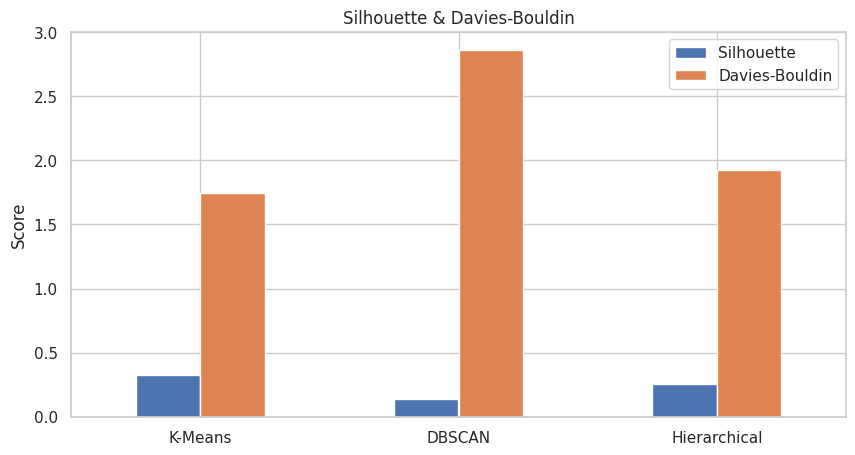
\includegraphics[width=0.9\linewidth]{expt-7_files/expt-7_21_0.png}
\end{center}

    \begin{center}
    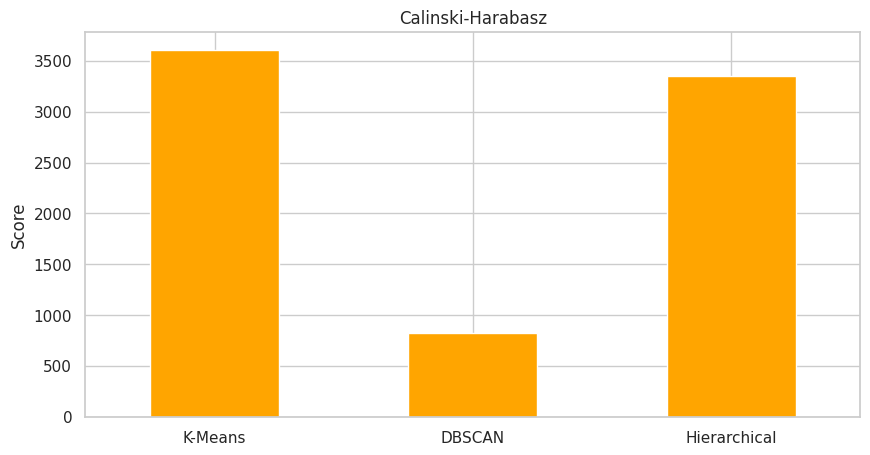
\includegraphics[width=0.9\linewidth]{expt-7_files/expt-7_21_1.png}
\end{center}
    
    \begin{tcolorbox}[breakable, size=fbox, boxrule=1pt, pad at break*=1mm,colback=cellbackground, colframe=cellborder]
\prompt{In}{incolor}{98}{\boxspacing}
\begin{Verbatim}[commandchars=\\\{\}]

\PY{c+c1}{\PYZsh{} External}
\PY{n}{external\PYZus{}metrics}\PY{o}{.}\PY{n}{plot}\PY{p}{(}\PY{n}{kind}\PY{o}{=}\PY{l+s+s1}{\PYZsq{}}\PY{l+s+s1}{bar}\PY{l+s+s1}{\PYZsq{}}\PY{p}{,} \PY{n}{figsize}\PY{o}{=}\PY{p}{(}\PY{l+m+mi}{10}\PY{p}{,}\PY{l+m+mi}{5}\PY{p}{)}\PY{p}{)}
\PY{n}{plt}\PY{o}{.}\PY{n}{title}\PY{p}{(}\PY{l+s+s1}{\PYZsq{}}\PY{l+s+s1}{External Clustering Metrics (vs True Labels)}\PY{l+s+s1}{\PYZsq{}}\PY{p}{)}
\PY{n}{plt}\PY{o}{.}\PY{n}{ylabel}\PY{p}{(}\PY{l+s+s1}{\PYZsq{}}\PY{l+s+s1}{Score}\PY{l+s+s1}{\PYZsq{}}\PY{p}{)}
\PY{n}{plt}\PY{o}{.}\PY{n}{xticks}\PY{p}{(}\PY{n}{rotation}\PY{o}{=}\PY{l+m+mi}{0}\PY{p}{)}
\PY{n}{plt}\PY{o}{.}\PY{n}{show}\PY{p}{(}\PY{p}{)}

\end{Verbatim}
\end{tcolorbox}

    \begin{center}
    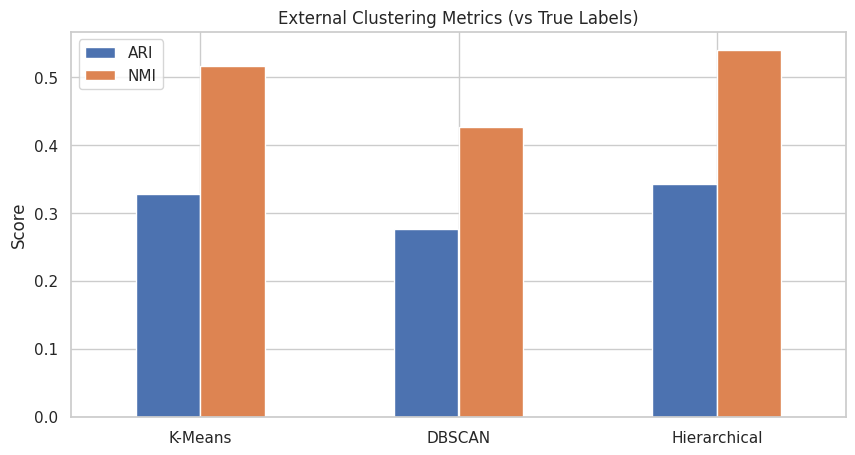
\includegraphics[width=0.9\linewidth]{expt-7_files/expt-7_22_0.png}
\end{center}

\vspace{0.8cm}
\section{Summary Tables}
\vspace{0.5cm}
\textbf{K-Means Elbow Method Results}
\begin{table}[H]
\centering
\caption{K-means Elbow Method Results}
\begin{tabular}{|c|c|c|}
\hline
\textbf{Number of Clusters (k)} & \textbf{WCSS (Inertia)} & \textbf{Silhouette Score} \\
\hline
2 & 2.336224e+06 & 0.396505 \\
3 & 2.081850e+06 & 0.327408 \\
4 & 1.976453e+06 & 0.165163 \\
5 & 1.875066e+06 & 0.130639 \\
6 & 1.818790e+06 & 0.108641 \\
7 & 1.776519e+06 & 0.111424 \\
8 & 1.737555e+06 & 0.073861 \\
\hline
\end{tabular}
\end{table}

\vspace{0.5cm}
\textbf{Evaluation Metrics (Internal and External)}
\begin{table}[H]
\centering
\caption{Clustering Algorithm Evaluation Metrics}
\begin{tabular}{|l|c|c|c|c|c|}
\hline
\textbf{Algorithm} & \textbf{Silhouette} & \textbf{Davies-Bouldin} & \textbf{Calinski-Harabasz} & \textbf{ARI} & \textbf{NMI} \\
\hline
K-means & 0.327408 & 1.745773 & 3605.263229 & 0.327923 & 0.516310 \\
DBSCAN & 0.141134 & 2.859937 & 825.391505 & 0.275990 & 0.426156 \\
Hierarchical & 0.254790 & 1.927494 & 3350.021309 & 0.342153 & 0.539664 \\
\hline
\end{tabular}
\end{table}

\vspace{1.0cm}
\section{Observations}
\begin{itemize}
    \item \textbf{Which algorithm produced the most meaningful clusters? Why?} \\
    Hierarchical Clustering appears to produce the most meaningful clusters. It has reasonably good internal metrics (Silhouette: 0.2548, Davies-Bouldin: 1.9275, Calinski-Harabasz: 3350.0) and the highest external metrics (ARI: 0.3422, NMI: 0.5397), indicating a better match with ground truth activities compared to K-Means and DBSCAN.

    \item \textbf{How sensitive was K-Means to the choice of k?} \\
    K-Means is quite sensitive to k. Silhouette score decreased consistently as k increased beyond 2-3, indicating that choosing too many clusters reduces cluster cohesion. The Elbow method suggested 2-3 clusters, which roughly aligns with the higher Silhouette scores, but the dataset has 6 true activity classes, showing that K-Means struggles to separate all activities clearly.

    \item \textbf{Did DBSCAN detect noise or small clusters effectively?} \\
    DBSCAN detected some noise points, but the clusters were not very meaningful at default parameters. Internal metrics were low (Silhouette: 0.1411, Davies-Bouldin: 2.8599, Calinski-Harabasz: 825.4), and external metrics (ARI: 0.2760, NMI: 0.4262) were worse than Hierarchical Clustering, showing it struggled to capture all activity classes effectively.

    \item \textbf{How does linkage choice (single/complete/ward) affect hierarchical clustering?} \\
    Using Ward’s linkage tends to produce compact, spherical clusters with better internal metrics, which is why Hierarchical Clustering with Ward’s method performed well in this assignment. Single linkage can create long chains (less compact clusters), while complete linkage can be sensitive to outliers.

    \item \textbf{Which internal metric best matched your visual intuition of cluster quality?} \\
    Silhouette Score best matched the visual cluster quality. Higher Silhouette values correlated with clusters that were visually well-separated in PCA/t-SNE plots, making it easier to assess cluster cohesion and separation.
\end{itemize}

\vspace{0.3cm}
\section{Learning Outcomes}
\begin{itemize}
    \item Understand and implement K-Means, DBSCAN, and Hierarchical Clustering algorithms on real datasets.
    \item Gain experience with cluster evaluation using internal metrics (Silhouette, Davies-Bouldin, Calinski-Harabasz) and external metrics (ARI, NMI).
    \item Interpret clustering results visually using PCA/t-SNE and understand how dimensionality reduction helps in analysis.
    \item Compare clustering algorithms and understand their strengths, weaknesses, and sensitivity to hyperparameters like k, $\epsilon$, minPts, and linkage methods.
    \item Develop skills to choose optimal hyperparameters using techniques like the Elbow method and metric-based evaluation.
\end{itemize}

\vspace{0.3cm}
\noindent
\textbf{GitHub Repository:} \\
\href{https://github.com/vidarshanaa15/ml-expt-7}{https://github.com/vidarshanaa15/ml-expt-7}

\end{document}

\end{document}